 \setlength{\baselineskip}{20pt}
 \interfootnotelinepenalty=10000
 \setlength{\tabcolsep}{5pt}
\chapter{数值实验设计及算法性能分析}
\label{cha:算法性能章}

% \tinytodo[inline]{修改章节导言}
\added[id=yrf]{本章将进行一系列实验以测试LR-ILS算法的性能,
以此验证算法的有效性,
特别关注于LR-ILS算法在解决大规模问题时的求解质量和求解时长。}
第\ref{sec:实验设计}节阐述了计算实验的平台与环境,
算法的参数取值以及数据来源等。
% % 第\ref{sec:数值实验}节详细分析了数值实验的结果,
% % 特别是对算法的性能进行了分析。
% 本节进行数值实验的
% 目的是分析算法求解大规模问题的能力,
% 以判断其求解现实问题的实用性。
第\ref{sec:综合性能}节对算法的整体性能进行了分析;
第\ref{sec:下界性能}节和第\ref{sec:上界性能}节分别分析了算法求解上下界的能力;
第\ref{sec:乘子性能}节讨论了不同拉格朗日乘子初始设置和更新策略的效果;
第\ref{sec:线性化优势}节讨论了模型线性化带来的求解增益效果;
第\ref{sec:算例结果}节展示了算例的选址结果及灵敏度分析结果;
最后,第\ref{sec:本章小结5}节总结了本章的主要工作。

\section{实验设计}
\label{sec:实验设计}
实验采用的计算平台的配置如下:
主频3.1Ghz的6核心12线程CPU(AMD 1600)搭配8Gb内存,
操作系统为Windows 10。
LR-ILS算法主程序由Matlab 2022b构建,
使用Python 3.9调用Gurobi 9.5.2进行建模。
为了加快程序运行速度,
额外使用了Matlab Coder将算法的关键步骤编译成二进制mex文件,
并在其中使用了多线程计算。

本文的第\ref{cha:LR算法}章LR-ILS算法设计考虑了一系列控制算法效果的参数,
经过多次的预实验,这些参数的取值如表\ref{table:参数取值}所示。
在预实验中,给定算法的参数初始值(根据经验预估),
每次调整固定算法的其他参数值,只调整一个参数,
直至在该参数下算法效果最好,
再更换其他参数进行调整。
\vspace{-2ex}
\begin{table}[!htb]\normalsize   %%\small是为了设置表格中的字体比正文小
\setlength{\abovecaptionskip}{1ex} 

\centering
\renewcommand\arraystretch{0.8}
\caption{LR-ILS算法参数取值\\Table~\ref{table:参数取值}~Parameter Setting for LR-ILS}
\small{
	\begin{tabular}{p{1.6cm}<{\centering} p{1.6cm}<{\centering} p{1.6cm}<{\centering} p{1.6cm}<{\centering} p{1.6cm}<{\centering} p{1.6cm}<{\centering} }
		% \begin{tabular}{c}{l}
		\toprule %[2pt]设置线宽  
		\multicolumn{2}{c}{LR} & \multicolumn{2}{c}{ILS} & \multicolumn{2}{c}{Gurobi}\\
		\cmidrule(r){1-2} \cmidrule(r){3-4} \cmidrule(r){5-6}
		参数   & 取值 & 参数  & 取值 & 参数  &  取值 \\
		\midrule %[2pt]
		$\alpha_0$      & 2      & $\theta_{sa}$  & 1.2    & MIPGap    & 0.00001\\
		$\alpha_{min}$  & 0.0001 & $T_{min}$      & 0.0001 & TimeLimit & 1000\\
		$\theta_{lr}$   & 1.05    & $\kappa_{ub}$  & 200\\
		$\kappa_{lb}$   & 10     & $\eta_{ils}$   & 10\\
		$\eta_{lr}$     & 3000  \\
		$\tau_{lim}$    & 1000(s)  \\
		$\xi$           & 0.01  \\
		\bottomrule %[2pt] 
	\end{tabular}
}
\vspace{-1ex}
\label{table:参数取值}
\end{table}

本节数值实验采用的数据来源于Snyder\cite{Snyder2005},
是选址研究的经典数据集。
该数据集包含了49、88、150个点的三套数据,
可在Snyder\cite{Snyder2005}的个人主页\footnote{https:\slash \slash coral.ise.lehigh.edu\slash larry\slash research\slash data-sets-for-reliability-models-for-facility-location-the-expected-failure-cost-case}下载。
原始数据为1990年美国房价普查数据,
包含了美国各个州的人口和房价数据。
学者们常使用该数据模拟节点选址中的固定成本和需求\cite{Daskin书,Snyder2005,yun2015,Cui2010}。
本文参考了Yun\cite{yun2017}的处理方法,
令客户的需求等于州人口数除以$10^5$,
节点的固定成本$f_j, \forall j \in J$等于房价的中位数,
令节点失效的概率等于$q_j = \rho e^{-f_j/200000},\forall j \in J$,
其中$\rho$是控制失效概率大小的参数,
惩罚成本$\pi = 10^4$, 客户最大尝试次数$R=5$。
此外,令客户点等于需求点,即$I=J$,
这样可以使图$G$中点的数量翻倍,
也不必再区分数据集中哪些点是客户点或是节点候选点。
令任意两点之间的距离等于大圆距离,
该距离的具体计算方法可见参考文献\cite{Snyder2005,Yongzhen,yun2015}。


\section{综合求解性能分析}
\label{sec:综合性能}

本节分析了算法的综合性能,
分为四个内容,
首先对比测试了LR-ILS算法求解不同规模、不同参数取值的数据的性能;
其次,对比Gurobi分析了求解时间和求解质量;
然后,分析了模型中两个重要参数$\rho$和$R$对LR-ILS求解性能的影响;
最后,通过上下界优化曲线直观展示了算法的迭代过程。
附录B展示了使用LR-ILS求解包含49、88、150个点的数据集的所有计算结果,
其中参数
$\rho$分别取0.01、0.05、0.1、0.2、0.3、0.4、0.5,
$R$分别取2至10。

\subsection{求解性能对比}
表\ref{table:LR与GRB}分别展示了LR-ILS算法和Gurobi求解器求解
49个点、88个点、150个点以及参数$\rho$不同取值的计算结果。
表\ref{table:LR与GRB}的所有实验均默认参数$R=5$,
其中gap值等于上下界之差除以上界,
相对差距等于LR-ILS得到的上界值减去Gurobi得到的上界值再除以二者之间的较小值,
因此相对差距为负时,LR-ILS获得了更优的上界,该值越小表明LR-ILS得到的结果越好。
相对速度等于Gurobi的求解时间除以LR-ILS的求解时间,
该值越大表明LR-ILS求解速度越快。

\begin{table}[hbt]
	\setlength{\abovecaptionskip}{-0.05cm} %调整图片caption与正文之间的间距,table同理。可自己调整。
	\setlength{\belowcaptionskip}{-0.2cm} 
	\centering
	\renewcommand\arraystretch{1}
	\caption{LR-ILS与Gurobi结果对比\\Table~\ref{table:LR与GRB}~Results for LR-ILS and Gurobi}
	\resizebox{\linewidth}{!}{
		\begin{tabular}{cccccccccc}
		\toprule %[2pt]设置线宽 
		\multirow{2}[0]{*}{数据集} & \multirow{2}[0]{*}{$\rho$} & \multicolumn{3}{c}{LR-ILS} & \multicolumn{3}{c}{Gurobi} 
		& \multirow{2}[0]{*}{\makecell[c]{相对\\差距(\%)}} & \multirow{2}[0]{*}{\makecell[c]{相对\\速度(倍)}} \\
		\cmidrule(r){3-5} \cmidrule(r){6-8}
		&       & 上界    & gap(\%) & 时间(s) & 上界    & gap(\%) & 时间(s) &       &  \\
		\midrule %[2pt]
		49    & 0.01  & 965061.90 & 0.99  & 0.21  & 965227.40 & 0.19  & 39.37 & -0.02 & 187.48 \\
		49    & 0.05  & 1018144.58 & 0.89  & 0.40  & 1021312.55 & 2.54  & 1000.00 & -0.31 & 2500.00 \\
		49    & 0.10  & 1076487.05 & 0.99  & 0.53  & 1077872.84 & 8.92  & 1000.00 & -0.13 & 1886.79 \\
		49    & 0.20  & 1198200.17 & 1.15  & 13.27 & 1224021.70 & 19.67 & 1000.00 & -2.16 & 75.36 \\
		88    & 0.01  & 1361557.62 & 1.00  & 0.76  & 1360245.50 & 1.16  & 1000.00 & 0.10  & 1315.79 \\
		88    & 0.05  & 1440083.62 & 0.99  & 1.18  & 1438341.99 & 6.09  & 1000.00 & 0.12  & 847.46 \\
		88    & 0.10  & 1527361.61 & 0.92  & 6.67  & 1544990.68 & 12.90 & 1000.00 & -1.15 & 149.93 \\
		88    & 0.20  & 1721135.80 & 2.70  & 98.52 & 1762412.99 & 23.85 & 1000.00 & -2.40 & 10.15 \\
		150   & 0.01  & 2176492.30 & 1.00  & 13.63 & -     & -     & 1000.00 & -     & - \\
		150   & 0.05  & 2279427.84 & 1.39  & 19.26 & -     & -     & 1000.00 & -     & - \\
		150   & 0.10  & 2391069.73 & 1.93  & 46.93 & -     & -     & 1000.00 & -     & - \\
		150   & 0.20  & 2611120.81 & 3.31  & 184.14 & -     & -     & 1000.00 & -    & - \\
		  \bottomrule %[2pt]   
	\end{tabular}%
	}
 \vspace{-2ex}
	\label{table:LR与GRB}
\end{table}%

数值结果表明
LR-ILS算法的显著优势在于能够在相对较短的时间内
获得质量较高的近似最优解,
具体分析如下:
首先,从求解的时间和速度进行分析,
除了第一组数据外,
Gurobi求解时长均到达了设置的最大运行时长,
并且150个点的问题全部没有在规定时间内得到结果。
相比之下,LR-ILS算法的求解时间显著优于Gurobi,
注意到该问题为NP-hard问题,
问题规模随节点数量增加而指数级增长。
因此在求解49个点的问题时,LR-ILS算法的求解效率是Gurobi的数千(百)倍,
求解88个点的问题时,求解效率退化至数百倍,
求解150个点的问题时,求解效率退化至数十倍,
表\ref{table:LR与GRB}中``相对速度(倍)''列展示了这种趋势。
相比Gurobi,
LR-ILS算法的求解速度具有显著优势。
在上界质量接近的情况下,
LR-ILS的求解时间更短。

其次,从求解的质量进行分析。
对比Gurobi,
对于49个点的全部算例,
LR-ILS获得了更加优质的上界;
对于88个点的部分算例,
LR-ILS的上界值略差于Gurobi,
但二者之间的相对差距($\le 0.12\%$)几乎可以忽略不计;
对于150个点的全部算例,
LR-ILS得到了上界的计算结果,
而Gurobi未能得到可行解。
Gurobi的上界质量和LR-ILS上界质量相差无几,
观察表中的gap值项,
除了第一组较为简单的数据集之外,
Gurobi的gap值均大于LR-ILS的gap值。
这表明证明上界的最优性方面,
Gurobi明显不如LR-ILS,
即拉格朗日松弛得到的下界优于Gurobi内置的线性松弛得到的下界。

\subsection{算例参数\texorpdfstring{$\rho$}{p}的影响}
尽管LR-ILS可以求解更复杂的问题并提供了优质下界,
但观察到无论是LR-ILS还是Gurobi,
求解问题所需的时长以及gap值都随参数取值的变化而变化。
% 为了探索参数对LR-ILS算法求解的影响,
% 本节的后续内容分析了在相等规模的情况下LR-ILS求解不同参数取值的算例性能,
% 以及讨论了产生这些现象的原因。
参数$\rho$的取值将影响LR-ILS算法的求解性能。
该参数控制节点的失效概率大小,
使得节点的失效概率接近$\rho$自身,
但由于节点的建设成本不一,
各个节点的失效概率也不相等。
随着参数$\rho$的增加,
模型的复杂程度提高,
LR-ILS算法的表现也越来越退化。
本节使用了49个点的算例进行测试,
$\rho$取0.1至0.9间隔为0.1的9个值,
$R$取2至10的整数,
求解时间及gap值随$\rho$变化
如图\ref{fig:result_time_rho}和图\ref{fig:result_gap_rho}所示。


\begin{figure}[ht] % use float package if you want it here
%\setlength{\abovecaptionskip}{-0.2cm} %调整图片caption与正文之间的间距,table同理。可自己调整。
\setlength{\belowcaptionskip}{-0.5cm} 
  \centering
  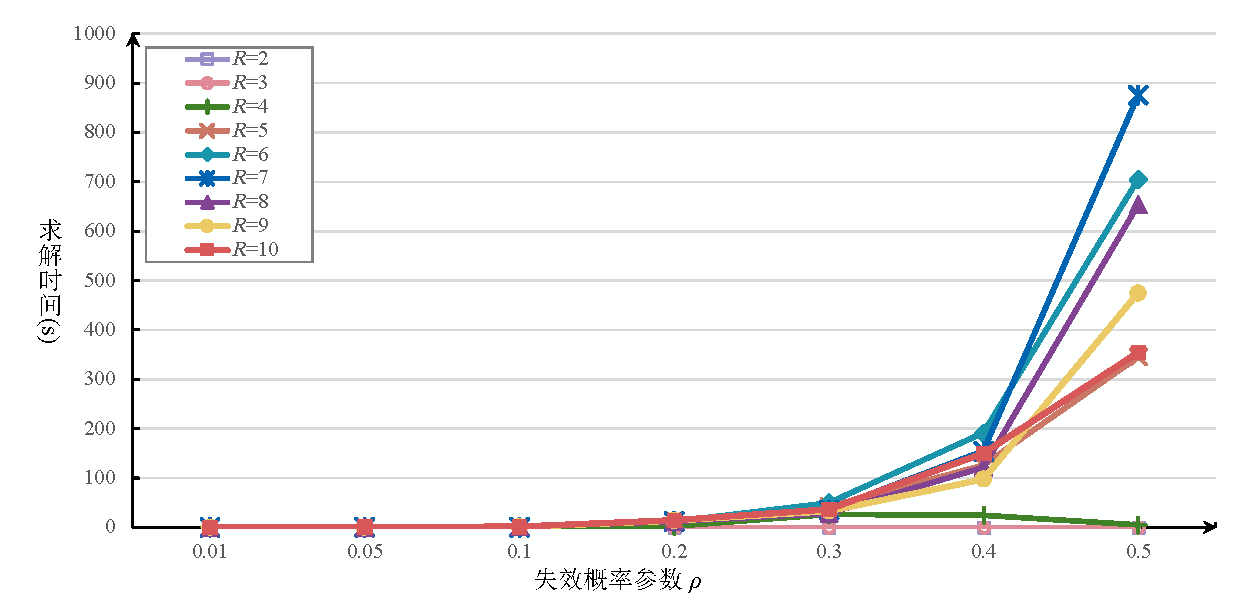
\includegraphics[width=0.9\textwidth]{figures/result_time_with_rho.pdf}
  \caption{LR-ILS算法求解时间随$\rho$的变化曲线\\Fig~\ref{fig:result_time_rho}~ Curves of LR computating time with respect to $\rho$}
  \label{fig:result_time_rho}
\end{figure}

\begin{figure}[ht] % use float package if you want it here
	%\setlength{\abovecaptionskip}{-0.2cm} %调整图片caption与正文之间的间距,table同理。可自己调整。
	\setlength{\belowcaptionskip}{-0.5cm} 
	  \centering
	  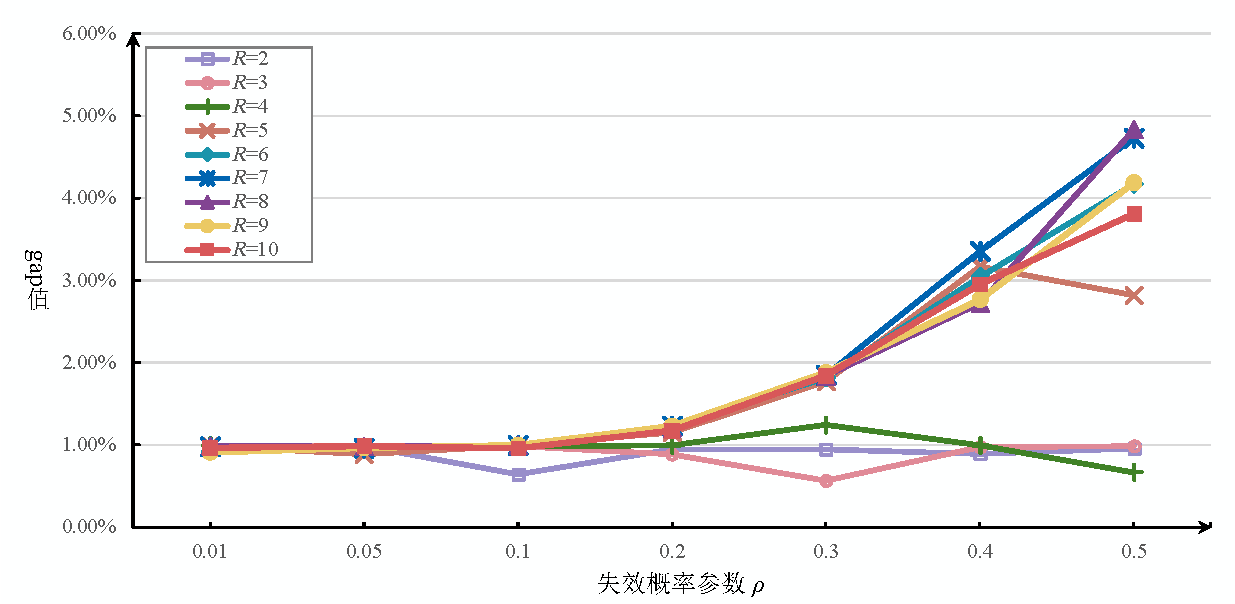
\includegraphics[width=0.9\textwidth]{figures/result_gap_with_rho.pdf}
	  \caption{LR-ILS算法求解gap随$\rho$的变化曲线\\Fig~\ref{fig:result_gap_rho}~ Curves of LR gap values with respect to $\rho$}
	  \label{fig:result_gap_rho}
\end{figure}


图\ref{fig:result_time_rho}和图\ref{fig:result_gap_rho}的横坐标轴表示参数$\rho$的变化范围,
纵坐标轴分别表示在此$\rho$取值下求解所需的计算时间以及结果的gap值,
不同颜色的线条表示不同$R$取值的结果。
首先分析求解时间与$\rho$的关系,
图\ref{fig:result_time_rho}中可见,参数$\rho$显著影响了求解的时间,
在大多数测试中,求解时间随参数$\rho$的增加而指数级增加,
特别是在$\rho=0.2$至0.5的区间内,
求解时间的增加变化十分明显。
这表明随着$\rho$取值变大,模型的复杂度提升,求解的难度随之增加。
求解难度提升的本质原因是随着节点失效概率增加,
求解客户试错序列的难度增加,
即安排客户不同等级的备用节点以充分降低惩罚成本,
以及在设施建设成本、期望运输成本以及惩罚成本三者之间权衡的难度增加。
这导致了算法的精确过程,例如DFS搜索过程的效率显著降低,
由于节点的失效概率增加,惩罚成本所占比重增加,
启发式不能提供一个优质的近似解导致DFS剪枝过程受影响,搜索次数、深度明显增加。
注意到在一些测试中,求解时长并不受$\rho$的显著影响,
这是因为这些测试的$R$的取值较小($\le 4$),
每个客户的常用节点和备用节点的指派任务较为简单(最优客户试错序列),
因此求解时长变化并不明显。
在$R \le 4$的情况下,
对于49个点的算例,LR-ILS算法可以在很短的时间内求解得到近似最优解。
对于$R$取值较大的情况,
LR-ILS也能在可接受的时间内求解得到一个结果。

其次,分析求解结果gap值随$\rho$的变化的关系。
与求解时间随$\rho$变化的情况类似,
在大部分测试中,
gap值同样随$\rho$增加而增加,
特别是在$\rho=0.2$至0.5的区间内的变化较为明显。
gap值证明了上界的最优性,
图\ref{fig:result_gap_rho}中所有的结果表明,
LR-ILS求解结果的gap值不超过5\%,
即LR-ILS算法求解49个客户点与49个备选点(或49个点以下)的问题时,
有能力得到一个在5\%误差内的近似最优解。
同样,$R \le 4$的测试结果中,
gap值受$\rho$变化的影响较小。
本文中LR-ILS算法设置停止准则的gap值为0.01,
因此一些测试的gap值只停留在1\%附近,
若改变算法参数,gap值有望进一步降低。

\subsection{算例参数\texorpdfstring{$R$}{R}的影响}
注意到在图\ref{fig:result_time_rho}和图\ref{fig:result_gap_rho}中,
并非$R$的值越大,求解的时间越久或gap值越高。
例如,在$\rho=0.5$时$R=7$的求解时间最长,
并且求解结果的gap值较高。
图\ref{fig:result_time_r}和图\ref{fig:result_gap_r}
从另一个角度分析了求解时间和gap值受参数$R$的影响程度。
图\ref{fig:result_time_r}和图\ref{fig:result_gap_r}
的横坐标表示$R$的不同取值,
纵坐标分别表示求解时间和gap值,
不同颜色的线条表示不同$\rho$的取值。

\begin{figure}[ht] % use float package if you want it here
	%\setlength{\abovecaptionskip}{-0.2cm} %调整图片caption与正文之间的间距,table同理。可自己调整。
	\setlength{\belowcaptionskip}{-0.5cm} 
	  \centering
	  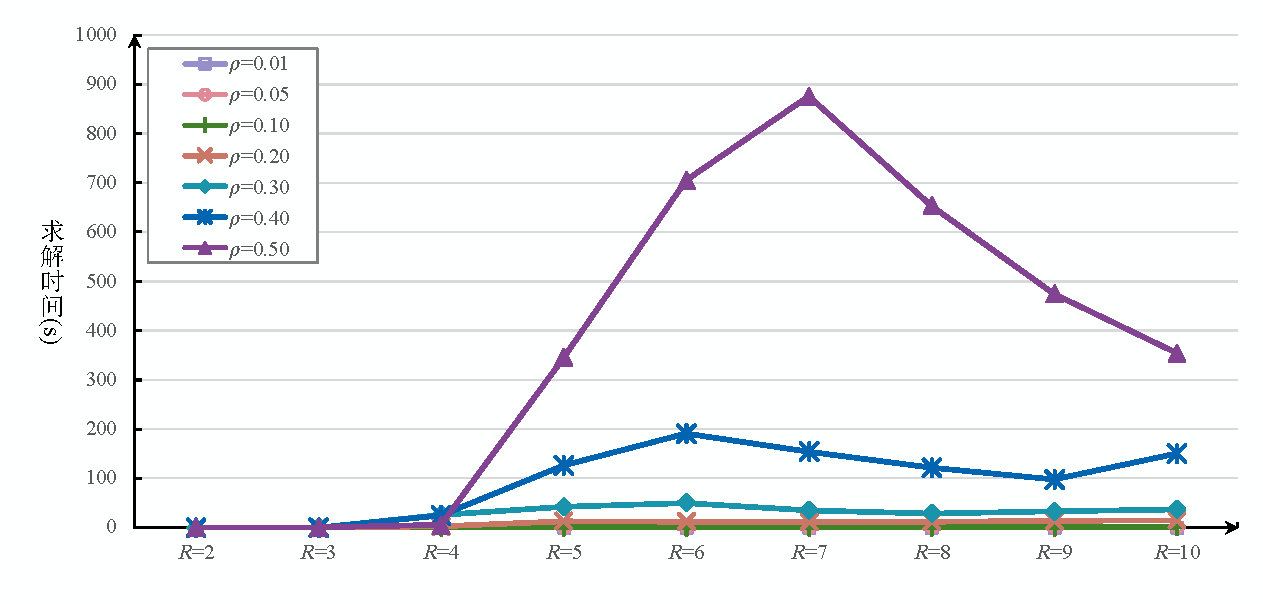
\includegraphics[width=0.9\textwidth]{figures/result_time_with_R.pdf}
	  \caption{LR-ILS算法求解时间随$R$的变化曲线\\Fig~\ref{fig:result_time_r}~ Curves of LR computating time with respect to $R$}
	  \label{fig:result_time_r}
\end{figure}
	
\begin{figure}[ht] % use float package if you want it here
	%\setlength{\abovecaptionskip}{-0.2cm} %调整图片caption与正文之间的间距,table同理。可自己调整。
	\setlength{\belowcaptionskip}{-0.5cm} 
		\centering
		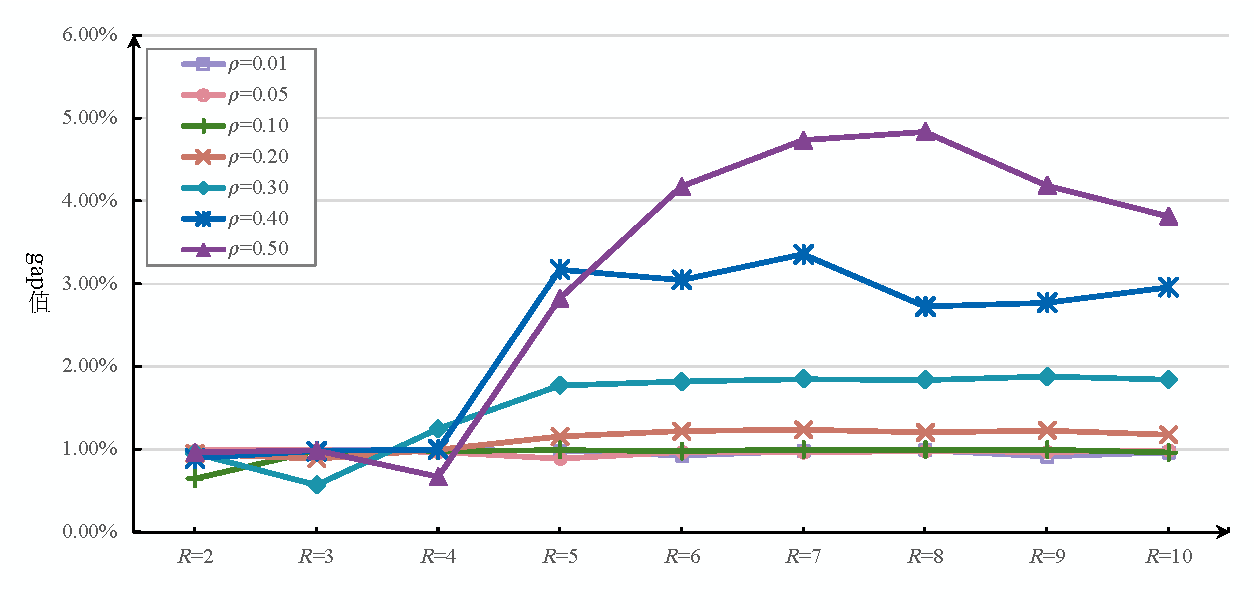
\includegraphics[width=0.9\textwidth]{figures/result_gap_with_R.pdf}
		\caption{LR-ILS算法求解gap随$R$的变化曲线\\Fig~\ref{fig:result_gap_r}~ Curves of LR gap values with respect to $R$}
		\label{fig:result_gap_r}
\end{figure}

在\ref{fig:result_time_r}和图\ref{fig:result_gap_r}中,
LR-ILS求解的时长以及gap值随参数$R$的增加
先上升后下降,这种趋势在$\rho$取值较大时更为明显。
产生该现象的原因是参数$R$和参数$\rho$对问题求解复杂程度的复合影响。
在$\rho$取值较大时,惩罚成本占比较高,
随着$R$不断增加,为了降低惩罚成本,
优化过程会为每个客户尽可能多地指派备用节点以降低惩罚成本,
因此求解模型的时间增加且gap值增加。
当$R$增加至一定值时,
求解时间或gap值增加到顶点。
对于49个点的算例来说,这个值是7或8。
随后,$R$值提升导致
客户前往接受惩罚的概率降低,
再增加$R$的值,
惩罚成本在总成本中的占比显著降低,
这反而降低了求解子问题的难度,
求解子问题时DFS剪枝策略又开始生效,
求解效率提升。
但是,随着$R$增加,问题更加复杂,
因此求解时间和gap值的表现也很难恢复至之前$R$取值较小的水平。

注意,上述分析单纯从数值角度出发,
在实际中,很少有节点伴随如此高的失效概率
($\rho = 0.5$时节点平均失效概率为35.14\%),
因此该算法仍可以求解现实问题。
本文同样给出了提高求解质量的途径:
参数调整方面,可适当增加LR的迭代次数,降低迭代步长比例因子,
算法设计方面,可改进上界获取的启发式,或开发求解试错序列问题的更有效算法。
即便LR-ILS算法求解失效概率较大的问题时,
获得的近似最优解gap不佳,
但该近似最优解仍优于Gurobi获得的解。
%TODO 令ILS连续出发值等于200 换图
\begin{figure}[htb] %这里使用的是强制位置,除非真的放不下,不然就是写在哪里图就放在哪里,不会乱动
	\centering  %图片全局居中
	\vspace{-0.35cm} %设置与上面正文的距离
	\subfigtopskip=2pt %设置子图与上面正文或别的内容的距离
	\subfigbottomskip=2pt %设置第二行子图与第一行子图的距离,即下面的头与上面的脚的距离
	\subfigcapskip=-5pt %设置子图与子标题之间的距离
	\subfigure[$\rho=0.01$]{
		\label{fig:lr_sub1}
		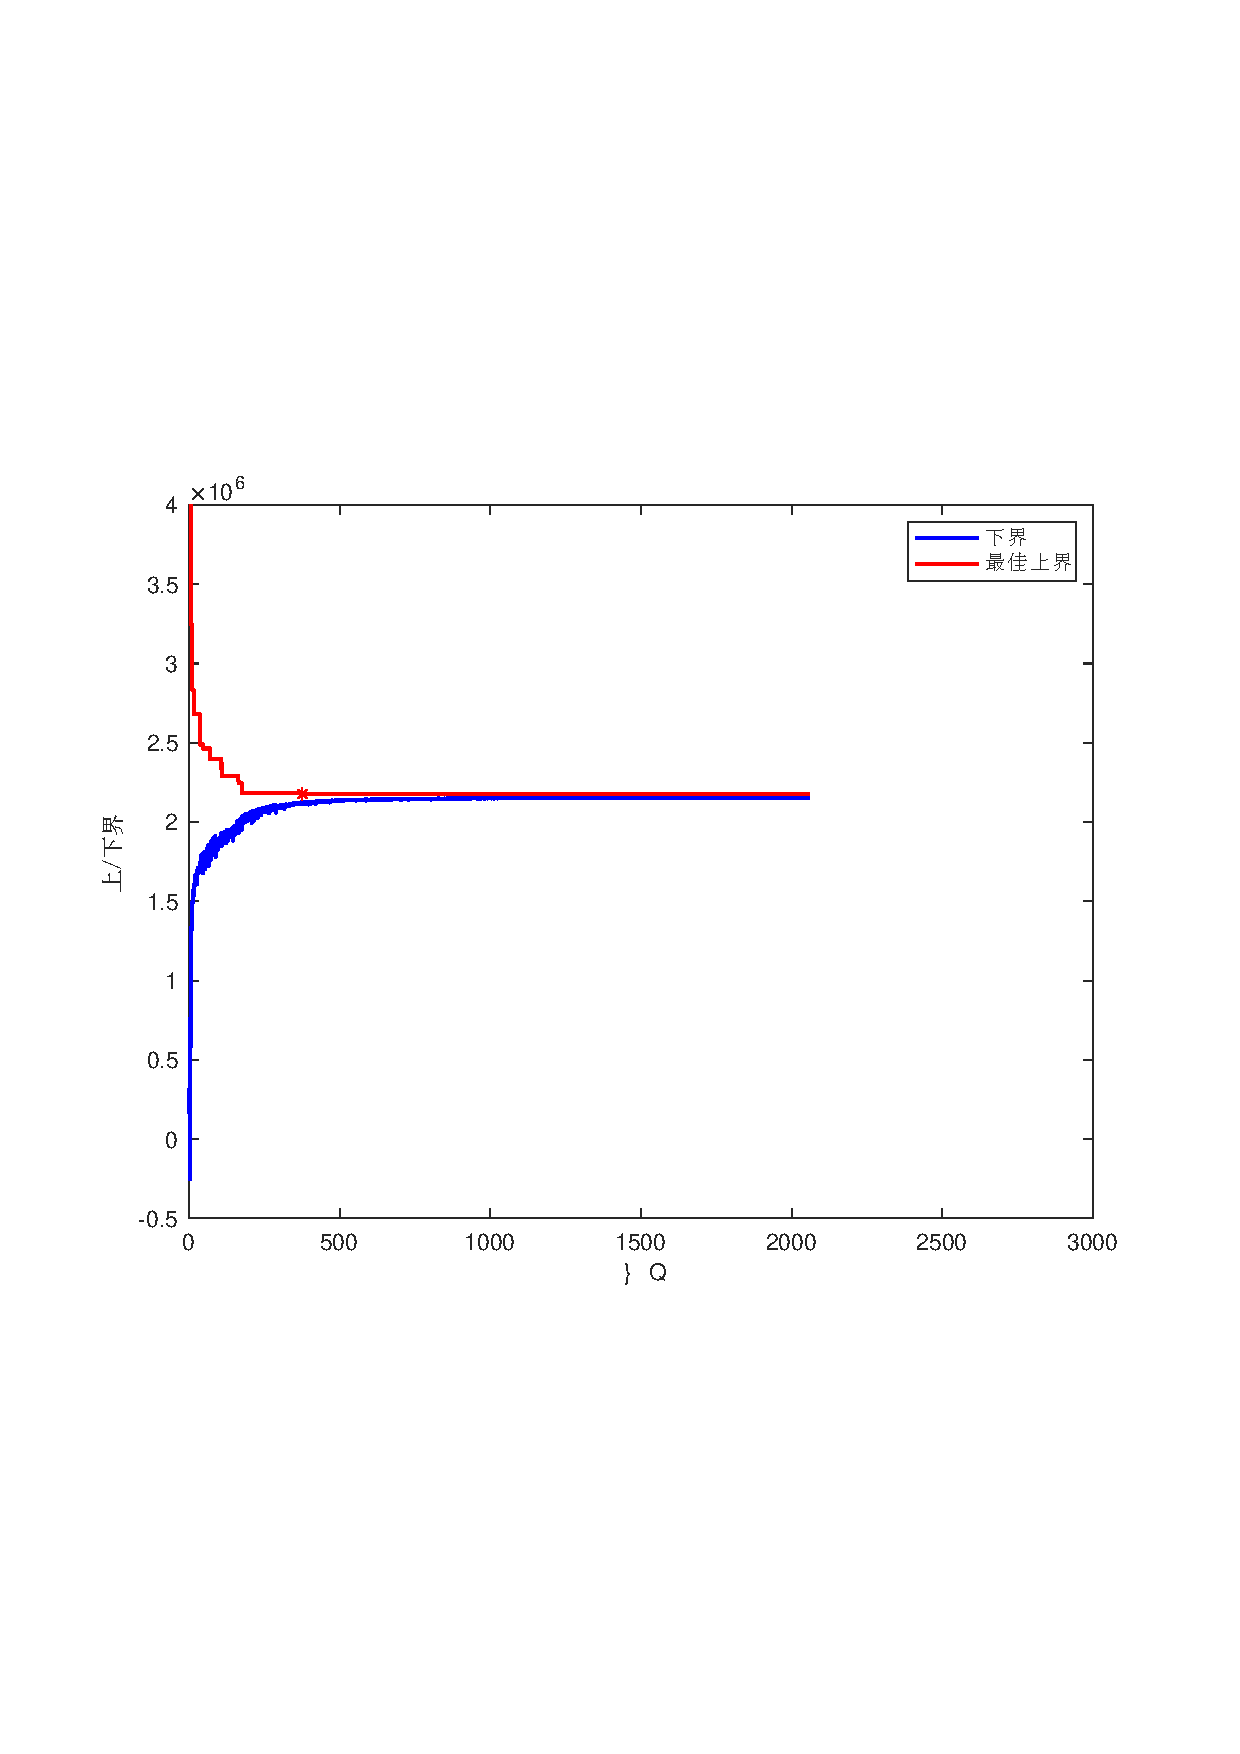
\includegraphics[width=0.47\linewidth]{figures/rslt_n150_rho0.01.pdf}}
	\quad %默认情况下两个子图之间空的较少,使用这个命令加大宽度
	\subfigure[$\rho=0.05$]{
		\label{fig:lr_sub2}
		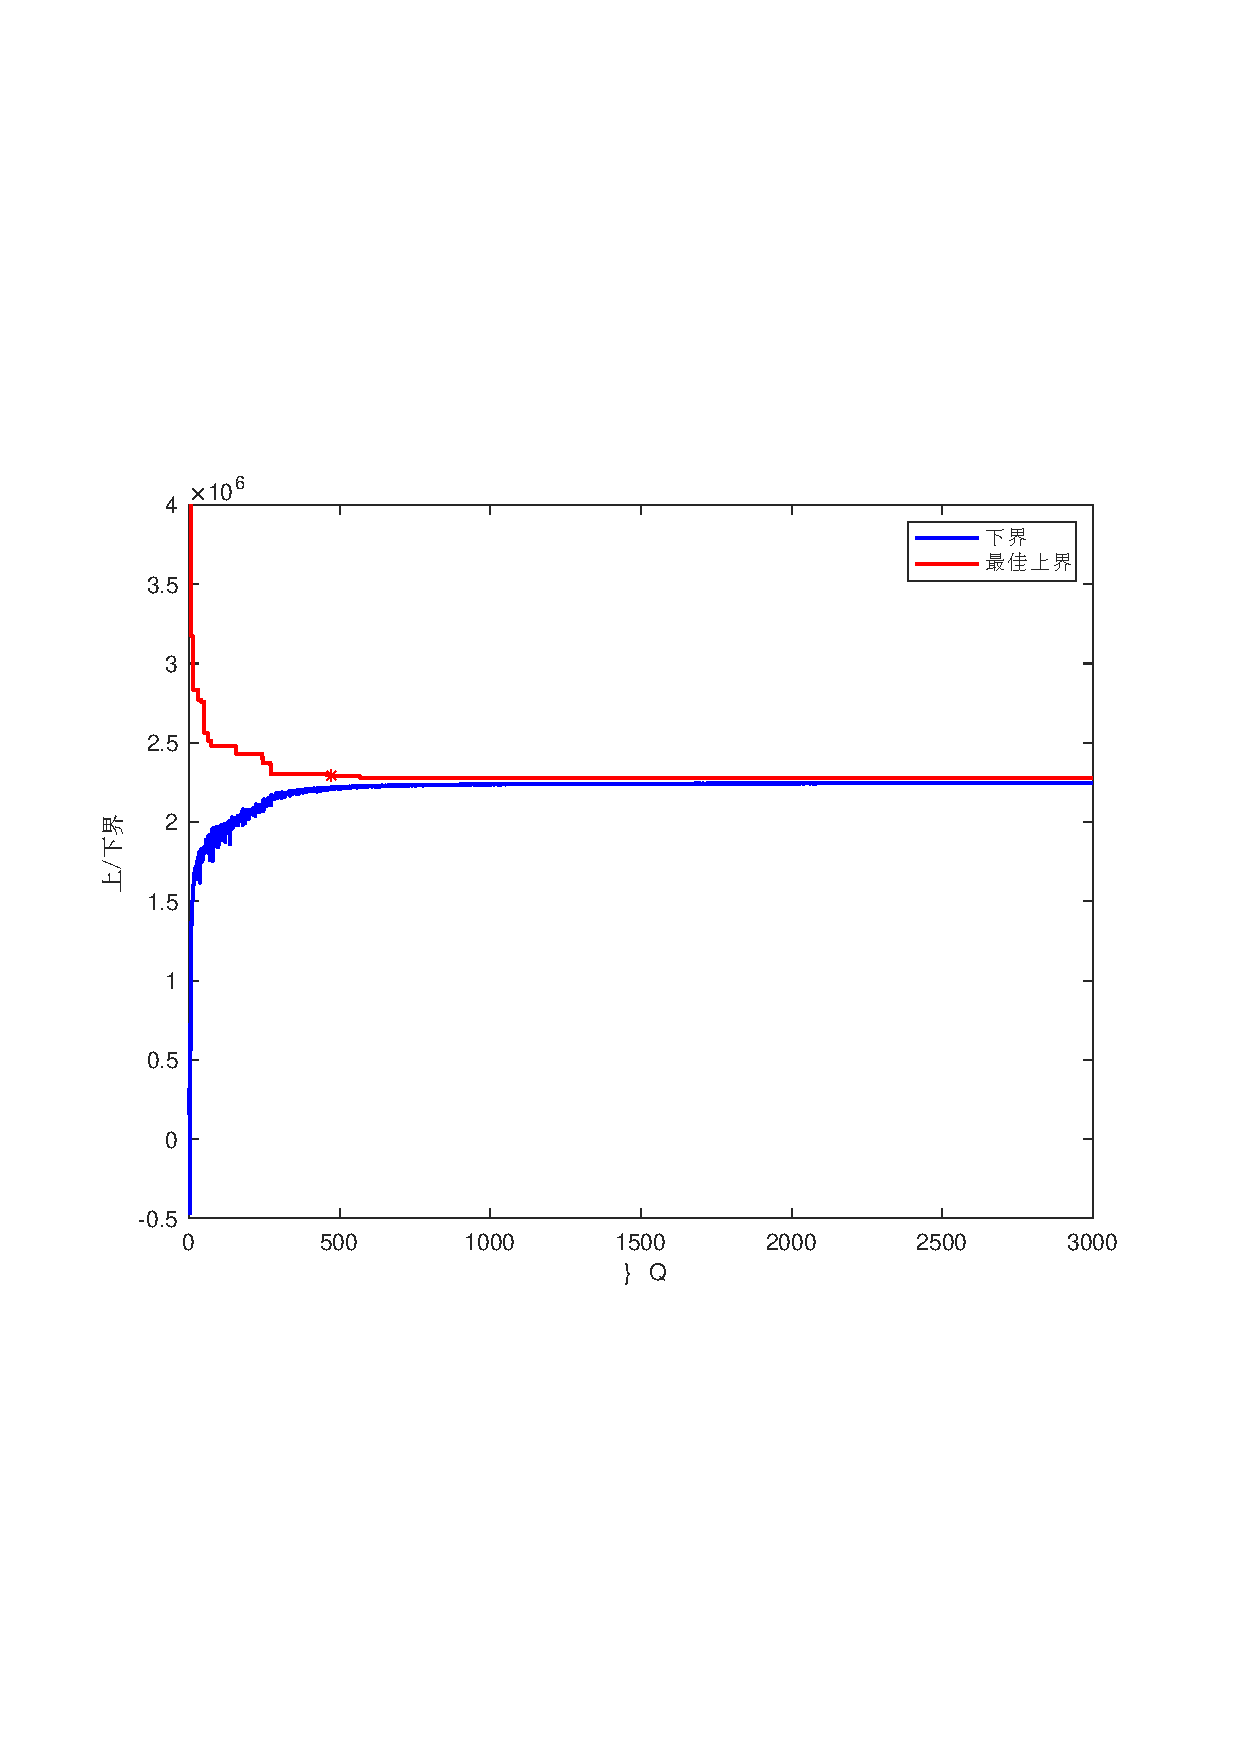
\includegraphics[width=0.47\linewidth]{figures/rslt_n150_rho0.05.pdf}}
	  %这里是空了一行,能够实现强制将四张图分成两行两列显示,而不是放不下图了再换行,使用\\也行。
	\subfigure[$\rho=0.10$]{
		\label{fig:lr_sub3}
		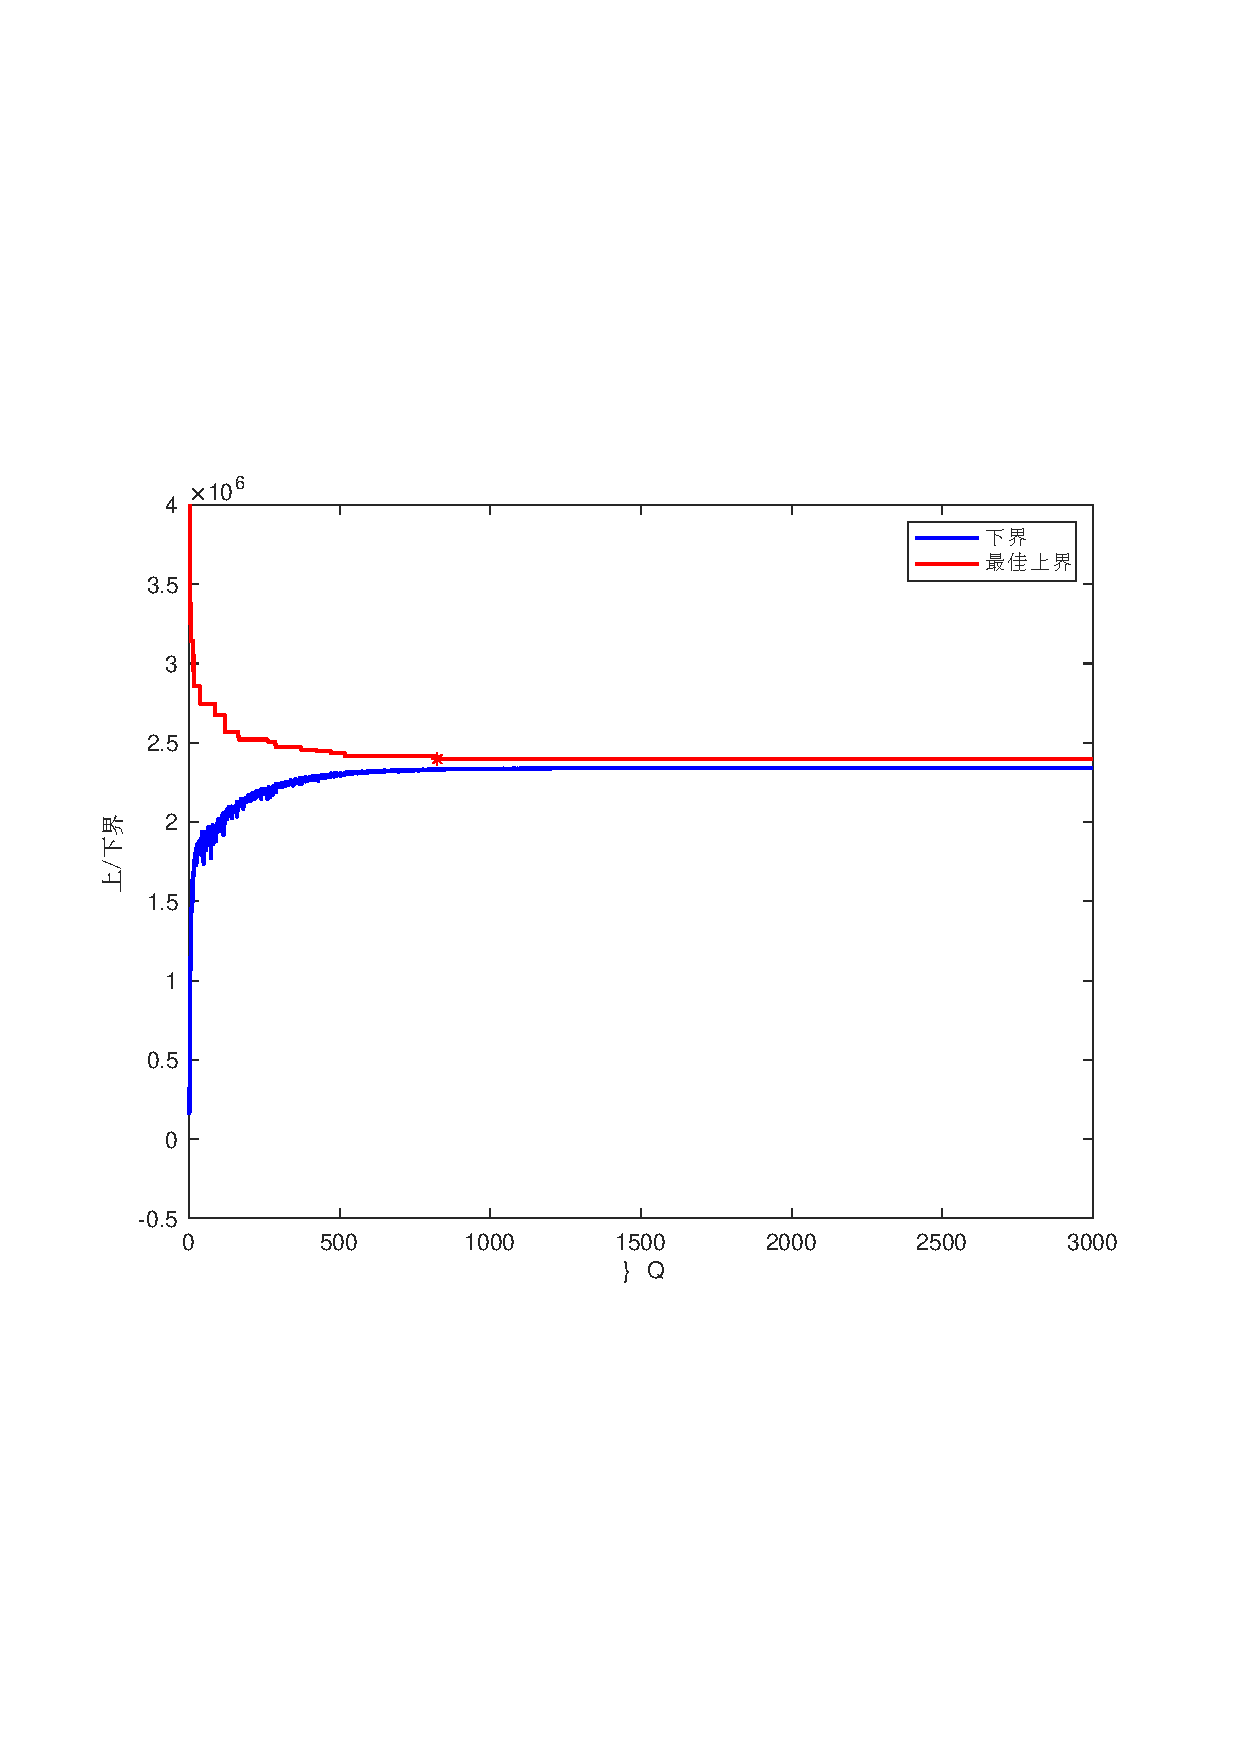
\includegraphics[width=0.47\linewidth]{figures/rslt_n150_rho0.1.pdf}}
	\quad
	\subfigure[$\rho=0.20$]{
		\label{fig:lr_sub4}
		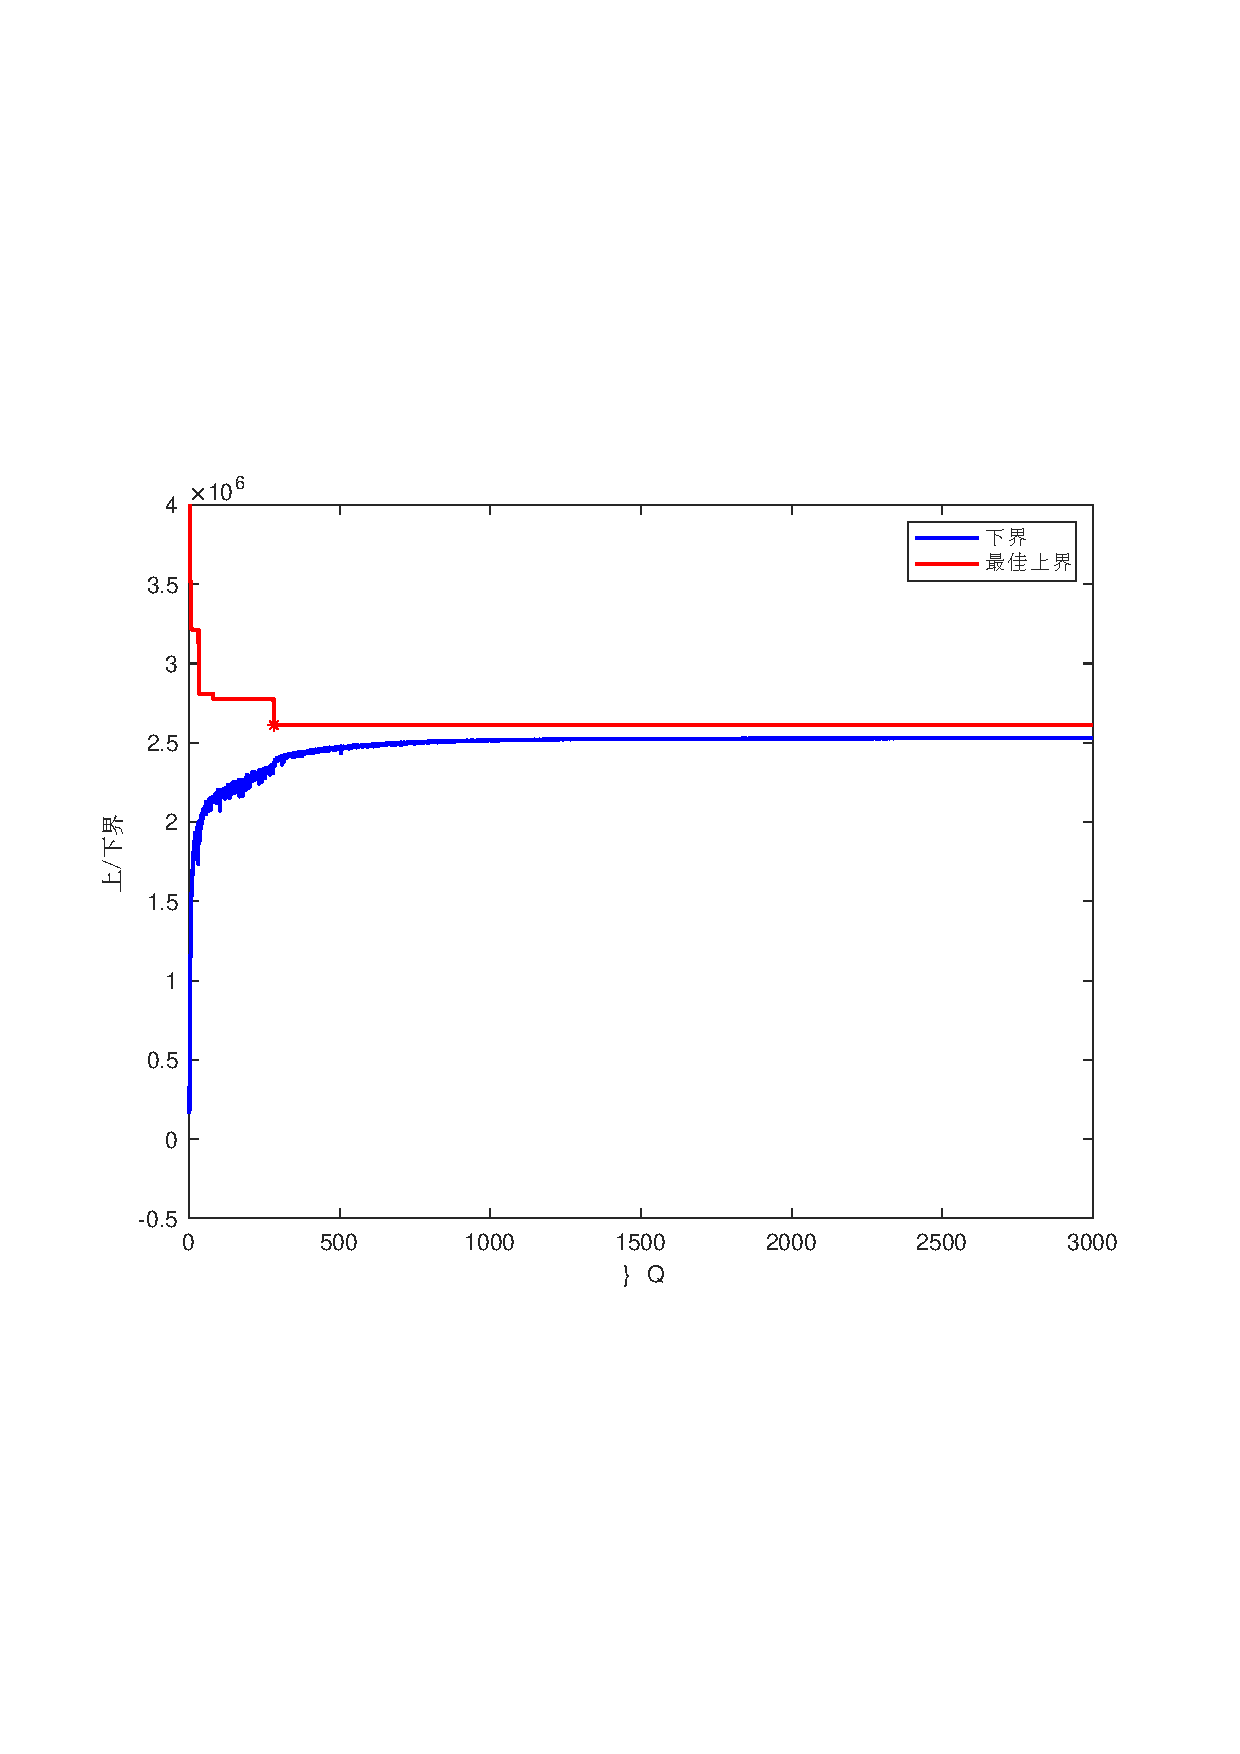
\includegraphics[width=0.47\linewidth]{figures/rslt_n150_rho0.2.pdf}}
	\caption{不同$\rho$取值的LR优化曲线\\Fig~\ref{fig:lr_curve_rho}~ LR optimization curves for different $\rho$}
	\label{fig:lr_curve_rho}
	\vspace{-0.35cm} %设置与上面正文的距离 
\end{figure}

\subsection{优化曲线}
最后,图\ref{fig:lr_curve_rho}直观展示LR-ILS算法优化过程,
使用了150个点的数据集,
默认参数$R=5$,
分别展示了了$\rho=0.01$、0.05、0.1、0.2,
不同取值的LR-ILS优化曲线。
图\ref{fig:lr_curve_rho}中,
横坐标表示迭代次数,
纵坐标表示上下界的取值;
红色的曲线表示最佳上界的变化,呈现阶梯状;
蓝色的曲线表示下界的变化,呈现锯齿状;
红色曲线上的标记表示ILS算子找到了更优的选址方案。
阶梯状上界的产生是因为LR-ILS每次迭代中仅记录最佳上界,
锯齿状下界的产生是因为迭代步长根据最佳上界值和当前下界值反复修正。
从图\ref{fig:lr_curve_rho}中可发现,算法的收敛过程相对较快,
可在500至1000次迭代内找到150个点的近似最优解,
然后下界不断提升证明其质量。
从图中可发现,
ILS可以改进上界,借助其搜索能力,
很容易根据当前上界解找到更优上界解,
进一步改进上界。
LR-ILS的大部分迭代过程在证明上界的质量,
优质上界主要由子模型RM$(\mu)_{sub1}$提供,
ILS算子的改进过程起到辅助作用。

\section{下界求解性能分析}
\label{sec:下界性能}
本节将分析算法中启发式与DFS算法求解下界解的性能,
由于构造启发式的时间复杂度优于插入启发式算法(第\ref{subsec:下界获取}节),
本节仅测试了插入启发式配合DFS算法求解下界的能力。
实验采用49个点的数据集,
$\rho$的值分别取$0.1$, $0.2$,$0.3$,
$R$值分别取2至10的整数,
拉格朗日乘子分别取全0、初始值与随机值,
其中随机值为0至30000之间的随机数。
仍采用Gurobi作为对比项,
Gurobi参数设置同表\ref{table:参数取值}一致。


测试结果如表\ref{table:下界性能}所示,
表中HEU表示仅使用启发式,
HEU-DFS表示使用启发式与DFS算法,
GRB表示使用Gurobi求解。
在测试得到的结果中,
HEU-DFS与GRB得到的结果为最优解,
HEU得到的结果为近似最优,
因此计算了HEU与最优值之间的差距,
并命名为gap*,求解时间的单位为秒,
HEU及HEU-DFS均为Matlab编码并转译生成的二进制文件,
采用了多线程计算。
表\ref{table:下界性能}中所有的结果均为$R$值分别取2至10的平均值,
该表的完整内容见附录B中的附表2。


\begin{table}[hbt]
	\small
	\setlength{\abovecaptionskip}{-0.05cm} %调整图片caption与正文之间的间距,table同理。可自己调整。
	\setlength{\belowcaptionskip}{-0.2cm} 
	\centering
	\renewcommand\arraystretch{1}
	\caption{下界求解性能\\Table~\ref{table:下界性能}~Performance on solving lower bound}
	% \resizebox{\linewidth}{!}{
		\begin{tabular}{crccccccc}
			\toprule
			\multirow{2}[1]{*}{\makecell[c]{乘子\\取值}} & \multicolumn{1}{c}{\multirow{2}[1]{*}{$\rho$}} & \multicolumn{2}{c}{HEU-DFS} & \multicolumn{3}{c}{HEU} & \multicolumn{2}{c}{GRB} \\
			\cmidrule(r){3-4} \cmidrule(r){5-7} \cmidrule(r){8-9}
			&       & 上界值   & 时间    & 上界值   & 时间(s) & gap*  & 上界值   & 时间(s) \\
			\midrule %[2pt]
			\multirow{3}[0]{*}{全零} & 0.1   & 224533.85 & 0.009 & 228752.63 & 0.001 & 0.42\% & 224532.63 & 85.260 \\
				  & 0.2   & 475214.35 & 0.012 & 493006.24 & 0.001 & 1.24\% & 475211.87 & 204.624 \\
				  & 0.3   & 756334.13 & 0.019 & 801825.67 & 0.000 & 2.68\% & 756331.82 & 388.021 \\
			\multirow{3}[0]{*}{初始} & 0.1   & 406887.38 & 0.002 & 411208.16 & 0.000 & 0.54\% & 406887.38 & 24.521 \\
				  & 0.2   & 702966.10 & 0.006 & 723855.37 & 0.000 & 1.92\% & 702966.10 & 120.713 \\
				  & 0.3	  & 1023301.45& 0.023 &1075474.89 & 0.000 & 3.23\% &1023301.45 & 349.158 \\ 
				%   & 0.3   & 513187.16 & 0.010 & 531729.61 & 0.001 & 1.36\% & 513185.96 & 164.628 \\
			\multirow{3}[1]{*}{随机} & 0.1   & 2077863.06 & 0.001 & 2082803.64 & 0.000 & 0.20\% & 2077863.06 & 15.280 \\
				  & 0.2   & 2570295.08 & 0.001 & 2600906.18 & 0.000 & 1.07\% & 2570295.08 & 15.393 \\
				  & 0.3   & 3066433.78 & 0.002 & 3140069.58 & 0.000 & 2.20\% & 3066433.78 & 22.739 \\
			\bottomrule
		\end{tabular}%
	% }
 	\vspace{-2ex}
	\label{table:下界性能}
\end{table}%

表\ref{table:下界性能}展示了采用三种方法求解得到的结果。
首先,分析三种方法的求解时间的差异。
尽管DFS算法并不是多项式时间算法,
但采用启发式搭配DFS算法得到的最优解的计算时间并不长,
并且随参数变动而变动的幅度较小。
而Gurobi的求解时间随参数变动而变动,
特别是随着$\rho$值升高,
Gurobi求解时间显著增长。
此外,拉格朗日乘子的取值对Gurobi的影响也十分大,
当乘子全为0时,Gurobi计算所有案例的平均时长为225.969s,
当乘子为初始值时,平均时长为164.797s,
当乘子取随机值时,平均时长为17.804s。
产生这种现象的原因是精确求解方法受参数影响较大。
当$R$值升高时,约束(\ref{eq:st_trytimes})变得松弛,
因此精确方法(Gurobi内置的各种Branch and Bound,Cutting Planes等方法)效果变差。
同理,随着$\rho$参数增加,节点失效概率参差不齐,
模型同样变得复杂。
拉格朗日乘子被视作访问节点的固定成本,
因此当乘子等于0时,求解器求解该模型相对困难,原因同上。
当乘子不等于0时,
精确方法可快速缩小可行域范围,
进而求解时间较短。
回到本文的启发式算法,
由于该算法是多项式时间算法,
因此求解时长随参数变动较小。
DFS算法虽然不是多项式时间算法,
但是剪枝过程大幅度缩短了计算所需的步骤,
与Gurobi相比是一种更有效地获取最优解的策略。

其次,分析三种方法求解结果的差异,
已知启发式搭配DFS算法和Gurobi可以获得最优解,
启发式方法可以获得近似解。
该启发式方法在$R$取值较大时、$\rho$取较小时,
表现良好。
并且受乘子取值的影响,
乘子不为零时表现良好。
分析该启发式的贪心策略可知,
算法每次将成本最小的节点增加至末尾。
当$R$值增加时,惩罚成本的比重逐渐被稀释,
使得贪心策略效果提升。
而$R$值较小时,贪心策略仅能考虑当前最优,
未能考虑最终惩罚成本的影响。
同理,当乘子不为零时,
乘子影响的贪心过程的决策,
进而提升了启发式的质量。
启发式方法获得的近似解总体质量较好(最大误差8.18\%,最小0.02\%,平均1.50\%),
但为了得到下界的最优解以证明上界的质量,
在本文算法仍使用了启发式搭配DFS的方式。
最后,值得注意的是,
尽管DFS和Gurobi都获得了最优解,
但在一些算例中,
Gurobi得到的值小于DFS方法得到的值。
经过排查,为决策变量$w_{ijk}$的值小于$10^{-6}$,
在Gurobi中认定为0。
有关Gurobi数值精度问题,
请参考Gurobi在线手册
\footnote{https:\slash \slash www.gurobi.com\slash documentation\slash 9.5\slash refman\slash guidelines\_for\_numerical\_i.html}。

\section{上界求解性能分析}
\label{sec:上界性能}

本文的第\ref{subsec:上界获取}节介绍了获取上界值的方法,
在给定选址方案$J^*$的前提下,
可很容易计算得到节点建设的固定成本,
计算客户的期望运输成本等于求解第\ref{subsec:subprob}节的客户试错序列问题。
第\ref{subsec:上界获取}节介绍的Dijkstra变种算法可以获得客户试错序列的近似解;
第\ref{subsec:上界获取}节提出可用DFS算法获得上界的最优值。
此外,还可使用Gurobi求解器求解模型的上界值。

本节对求解上界的性能进行了测试,
分别使用了Dijkstra变种算法(本节简称为DIJK),
Dijkstra变种算法搭配DFS算法(本节简称为DIJK-DFS),
以及Gurobi求解器(本节简称为GRB)求解了49个点的不同算例。
已知选址方案$J^*$中设施的个数显著影响算法求解时长,
因此,本节分别测试了10,20,30,40个点的选址方案,
参数$\rho$取值0.1,0.2,0.3,
参数$R$取值为大于等于2小于等于10的整数。
测试结果如表\ref{table:上界性能}所示,
表中近似解与最优之间的差距命名为gap*。
求解时间单位为秒,
DIJK算法与DIJK-DFS算法均为Matlab编码并转译成C++二进制文件,
采用了多线程计算。
表\ref{table:上界性能}中所有的结果均为$R$值分别取2至10的平均值,
该表的完整内容见附录B中的附表3。
 

\begin{table}[hbt]
	\small
	\setlength{\abovecaptionskip}{-0.05cm} %调整图片caption与正文之间的间距,table同理。可自己调整。
	\setlength{\belowcaptionskip}{-0.2cm} 
	\centering
	\renewcommand\arraystretch{1}
	\caption{上界求解性能\\Table~\ref{table:上界性能}~Performance on solving upper bound}
		\begin{tabular}{crccccccc}
			\toprule
			\multirow{2}[1]{*}{\makecell[c]{$|J^*|$}} & \multicolumn{1}{c}{\multirow{2}[1]{*}{$\rho$}} & \multicolumn{2}{c}{DIJK-DFS} & \multicolumn{3}{c}{DIJK} & \multicolumn{2}{c}{GRB} \\
			\cmidrule(r){3-4} \cmidrule(r){5-7} \cmidrule(r){8-9}
			&       & 上界值   & 时间    & 上界值   & 时间(s) & gap*  & 上界值   & 时间(s) \\
			\midrule %[2pt]
			\multirow{3}[0]{*}{10} 	& 0.1   & 1611587.91 & 0.001 & 1640555.97 & 0.006 & 1.90\% & 1611590.82 & 5.111 \\
									& 0.2   & 1925003.60 & 0.001 & 2011904.94 & 0.001 & 4.68\% & 1925001.32 & 5.803 \\
									& 0.3   & 2287526.81 & 0.001 & 2472292.62 & 0.001 & 8.35\% & 2287525.39 & 6.340 \\
	 		\multirow{3}[0]{*}{20} 	& 0.1   & 2067339.22 & 0.001 & 2072951.15 & 0.001 & 0.22\% & 2067342.67 & 10.999 \\
									& 0.2   & 2335167.39 & 0.002 & 2371565.20 & 0.001 & 1.39\% & 2335168.60 & 11.597 \\
									& 0.3   & 2639304.64 & 0.002 & 2750515.28 & 0.001 & 4.01\% & 2639302.63 & 14.668 \\
	  		\multirow{3}[0]{*}{30} 	& 0.1   & 2752865.35 & 0.003 & 2761269.07 & 0.001 & 0.22\% & 2752853.58 & 19.238 \\
									& 0.2   & 3011919.92 & 0.006 & 3097686.57 & 0.001 & 2.61\% & 3011907.14 & 25.567 \\
									& 0.3   & 3305273.39 & 0.006 & 3490345.05 & 0.001 & 5.16\% & 3305262.35 & 45.998 \\
	  		\multirow{3}[0]{*}{40} 	& 0.1   & 3323545.36 & 0.004 & 3331937.55 & 0.001 & 0.20\% & 3323545.56 & 48.869 \\
									& 0.2   & 3575894.34 & 0.006 & 3640638.02 & 0.001 & 1.66\% & 3575893.29 & 84.519 \\
									& 0.3   & 3858144.43 & 0.017 & 4031583.03 & 0.001 & 4.25\% & 3858140.97 & 156.080 \\
			\bottomrule
		\end{tabular}%
 	\vspace{-2ex}
	\label{table:上界性能}
\end{table}%


表\ref{table:上界性能}展示了使用三种方法求解上界的结果,
从求解时间的角度分析,
对比Gurobi求解器,
DIJK算法以及DIJK-DFS算法具有显著优势。
对于所有算例,上述两种算法可以在0.1秒内给出上界值,
而Gurobi虽然可以获得上界值,
但求解时间明显与这两种算法不在同一数量级
(最小差距1131.29倍,最大差距63136.36倍,详见附表3)。
并且Gurobi的求解时间随参数变动而变动,
$|J^*|$越大、参数$\rho$越大、参数$R$越大,
则模型越复杂,导致Gurobi求解时间越长。
最短可在几秒内完成简单算例的求解,
最长需要几分钟。
DIJK算法以及DIJK-DFS算法求解时间则非常稳定,
最长不超过0.1秒。
Gurobi求解时长随参数变化的原因已在第\ref{sec:下界性能}节分析。

已知在本测试中,
Gurobi和DIJK-DFS获得上界的最优值,
但DIJK算法只能获得近似值。
表\ref{table:上界性能}的gap*列
展示了该算法获得的近似上界值和最优值之间的相对差距,
在$R$值较大时,DIJK算法得到的解质量较好。
但在$R$值较小时,DIJK算法算法表现劣化。
DIJK算法是基于Dijkstra算法进行了问题的适配,
但保留了Dijkstra算法永久标号的主要想法,
所以不可修改的标号将在$R$值较小时生成质量欠佳的决策,
进而影响解的质量。
当$R$值较大时,即便初始步骤生成的路径质量欠佳,
可通过后续决策降低惩罚成本的比重。
即便DIJK算法求解$R$值较小的问题的效果较差,
但DFS算法在$R$值较小时因搜索深度较小而展现了良好的性能。

综上,求解上界的Dijkstra变种算法在求解$R$值较小的问题时,
得到的上界质量较差,但DFS算法的搜索深度较浅,
可快速基于Dijkstra变种算法的解获得最优解。
在$R$值较大时,Dijkstra变种算法得到的上界质量较好,
为DFS算法提供了一个质量较好的已知解,
加速了DFS中剪枝的过程。
两种算法优势互补,使求解上界的过程十分有效。


\section{乘子更新效果讨论}
\label{sec:乘子性能}
本文的第\ref{subsec:乘子更新}小节阐述了拉格朗日乘子初始设置以及乘子更新的方法,
本节将对比多种乘子初始化方法以及两种乘子更新方法的不同效果。
为了显著体现不同拉格朗日乘子设置产生的效果,
本节使用了相对较小的49个点的数据集进行实验,
对比分析拉格朗日优化曲线的收敛性。
在本节中,默认设置参数$R=5$,
参数$\rho$分别取值0.05、0.1、0.2、0.3。
为了消除其他因素的干扰,
本节的所有测试均关闭了ILS算子。

\begin{figure}[!t] %这里使用的是强制位置,除非真的放不下,不然就是写在哪里图就放在哪里,不会乱动
	\centering  %图片全局居中
	\vspace{-0.35cm} %设置与上面正文的距离
	\subfigtopskip=2pt %设置子图与上面正文或别的内容的距离
	\subfigbottomskip=2pt %设置第二行子图与第一行子图的距离,即下面的头与上面的脚的距离
	\subfigcapskip=-5pt %设置子图与子标题之间的距离
	\subfigure[$\rho=0.05$]{
		\label{fig:mp_sub1}
		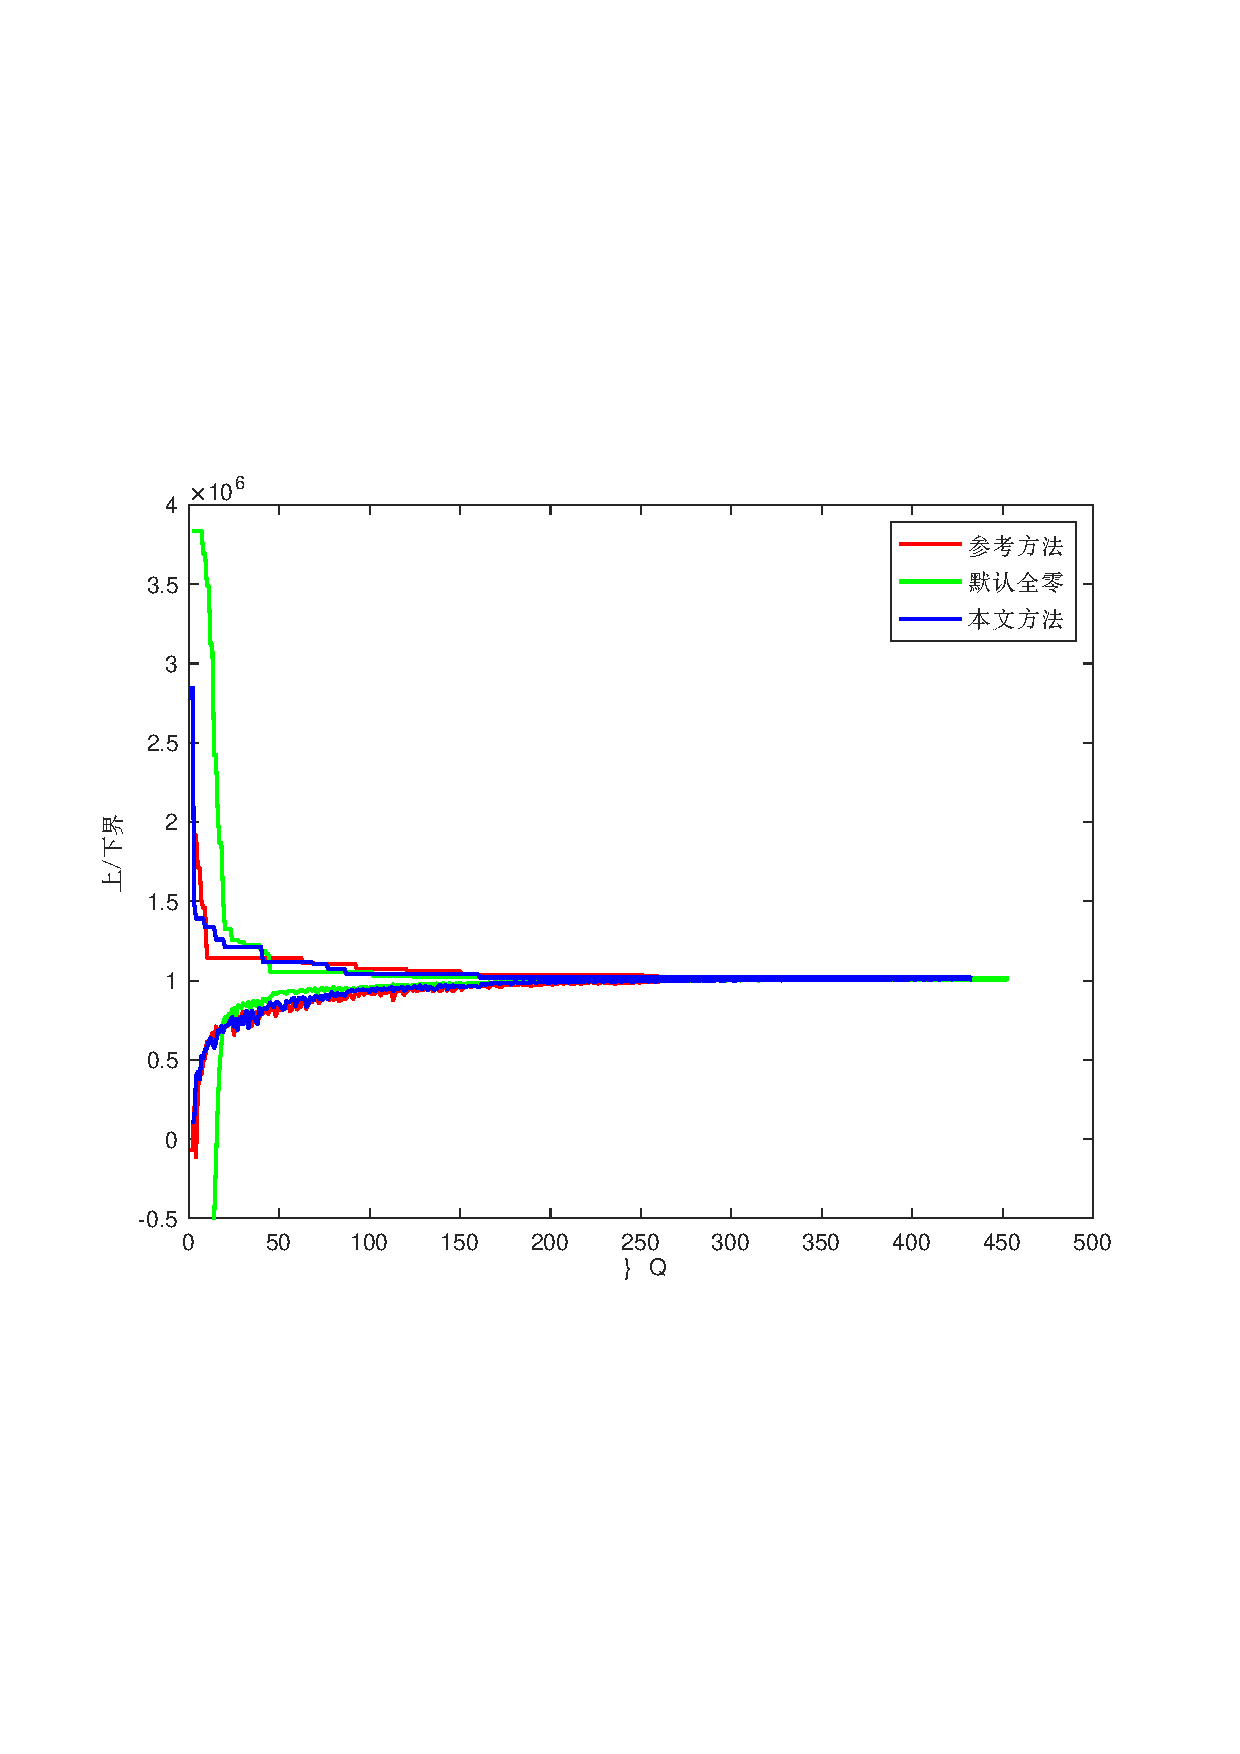
\includegraphics[width=0.47\linewidth]{figures/result_mp_rho0.05.pdf}}
	\quad %默认情况下两个子图之间空的较少,使用这个命令加大宽度
	\subfigure[$\rho=0.1$]{
		\label{fig:mp_sub2}
		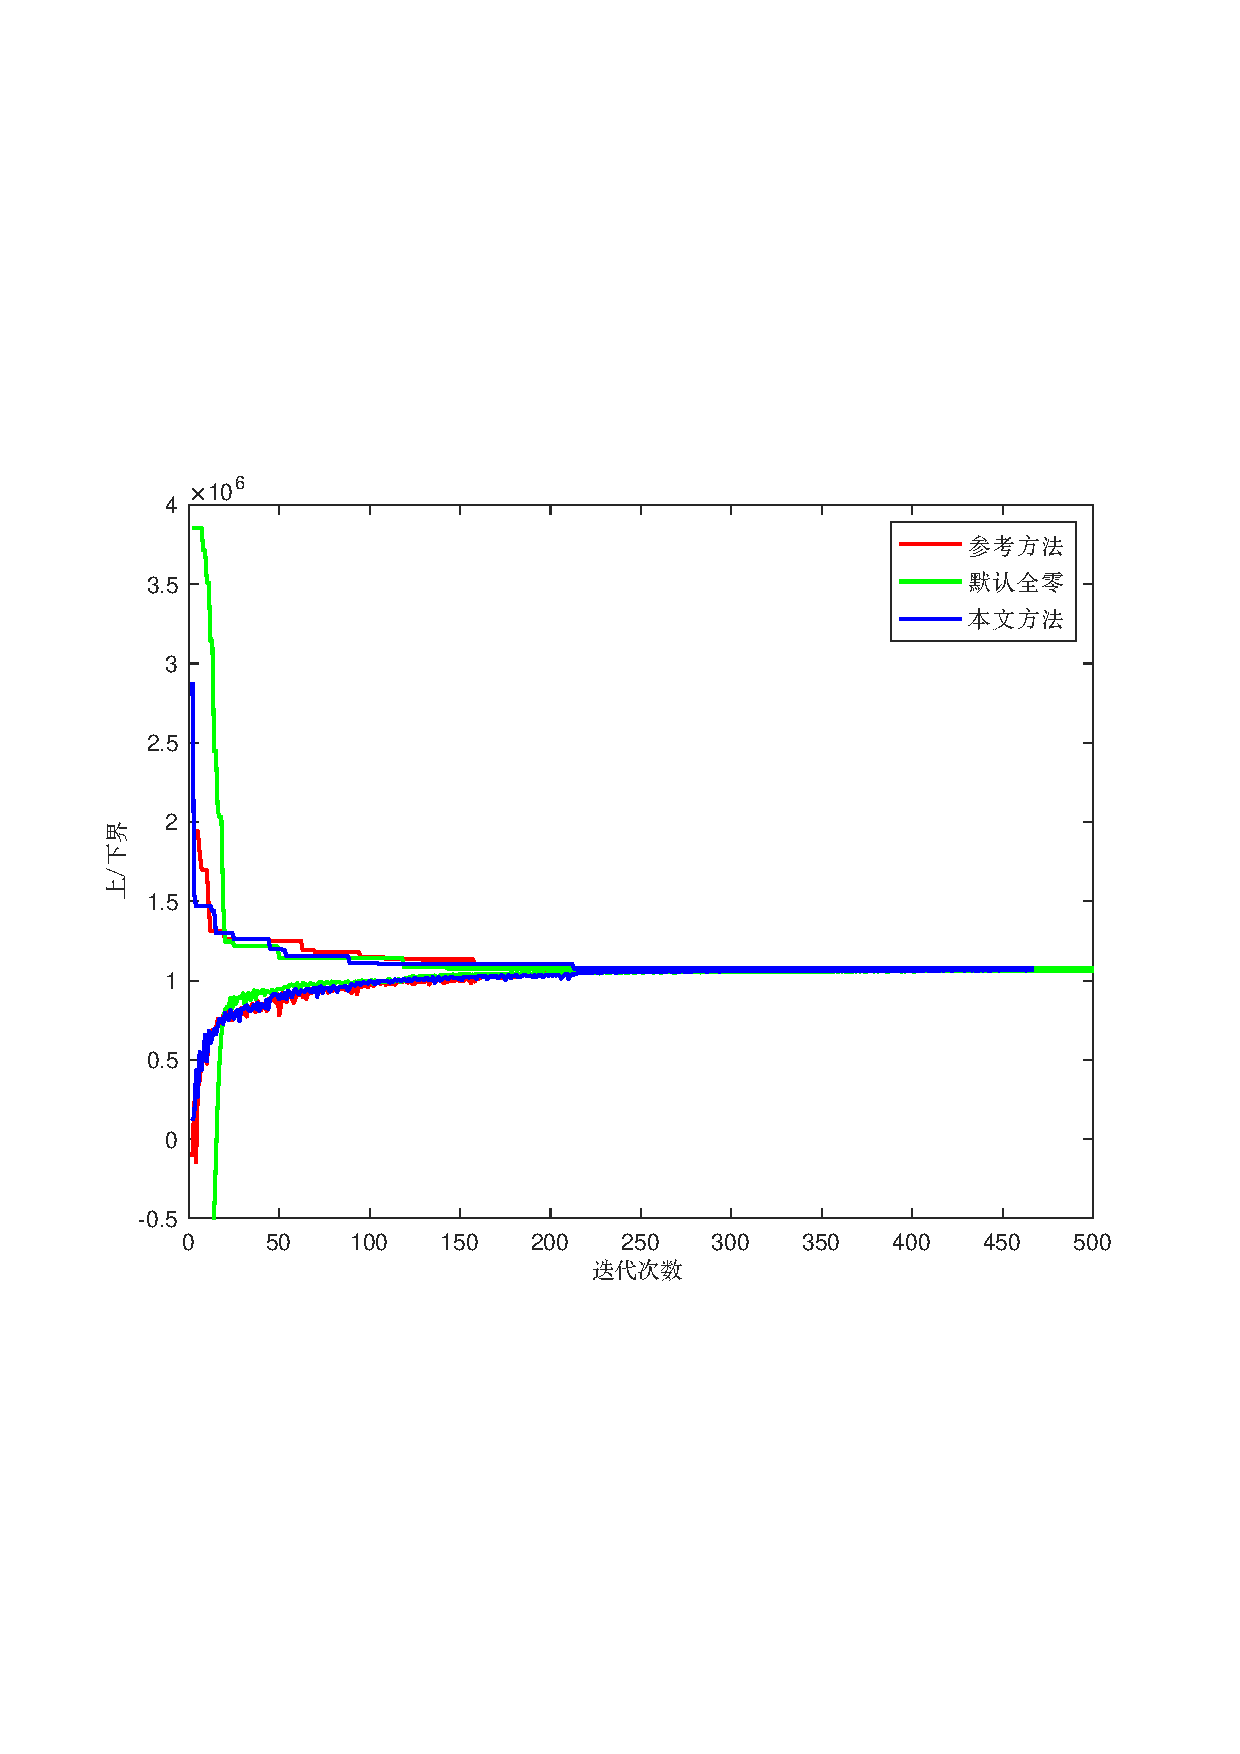
\includegraphics[width=0.47\linewidth]{figures/result_mp_rho0.1.pdf}}
	  %这里是空了一行,能够实现强制将四张图分成两行两列显示,而不是放不下图了再换行,使用\\也行。
	\subfigure[$\rho=0.2$]{
		\label{fig:mp_sub3}
		% \includegraphics[width=0.47\linewidth]{figures/result_mp_rho0.2.eps}}
		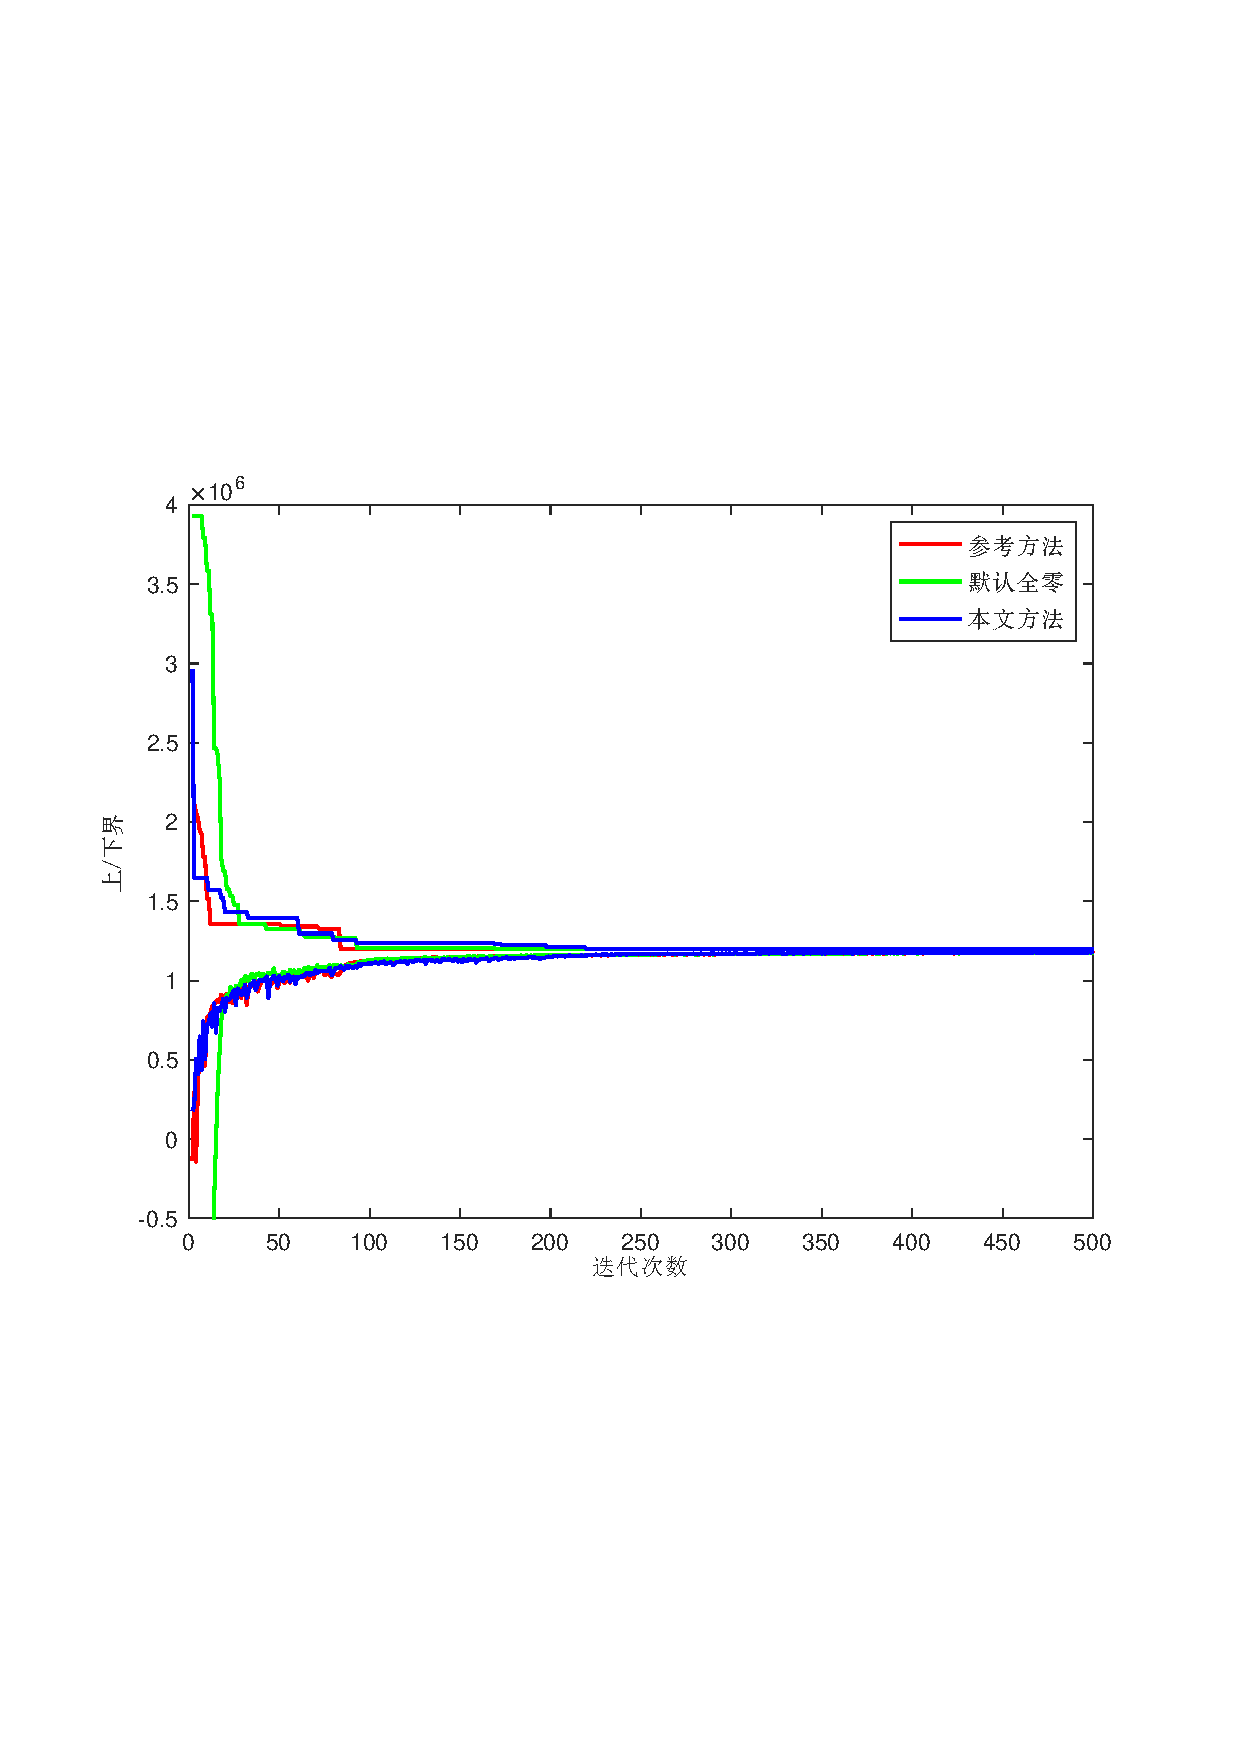
\includegraphics[width=0.47\linewidth]{figures/result_mp_rho0.2.pdf}}
	\quad
	\subfigure[$\rho=0.3$]{
		\label{fig:mp_sub4}
		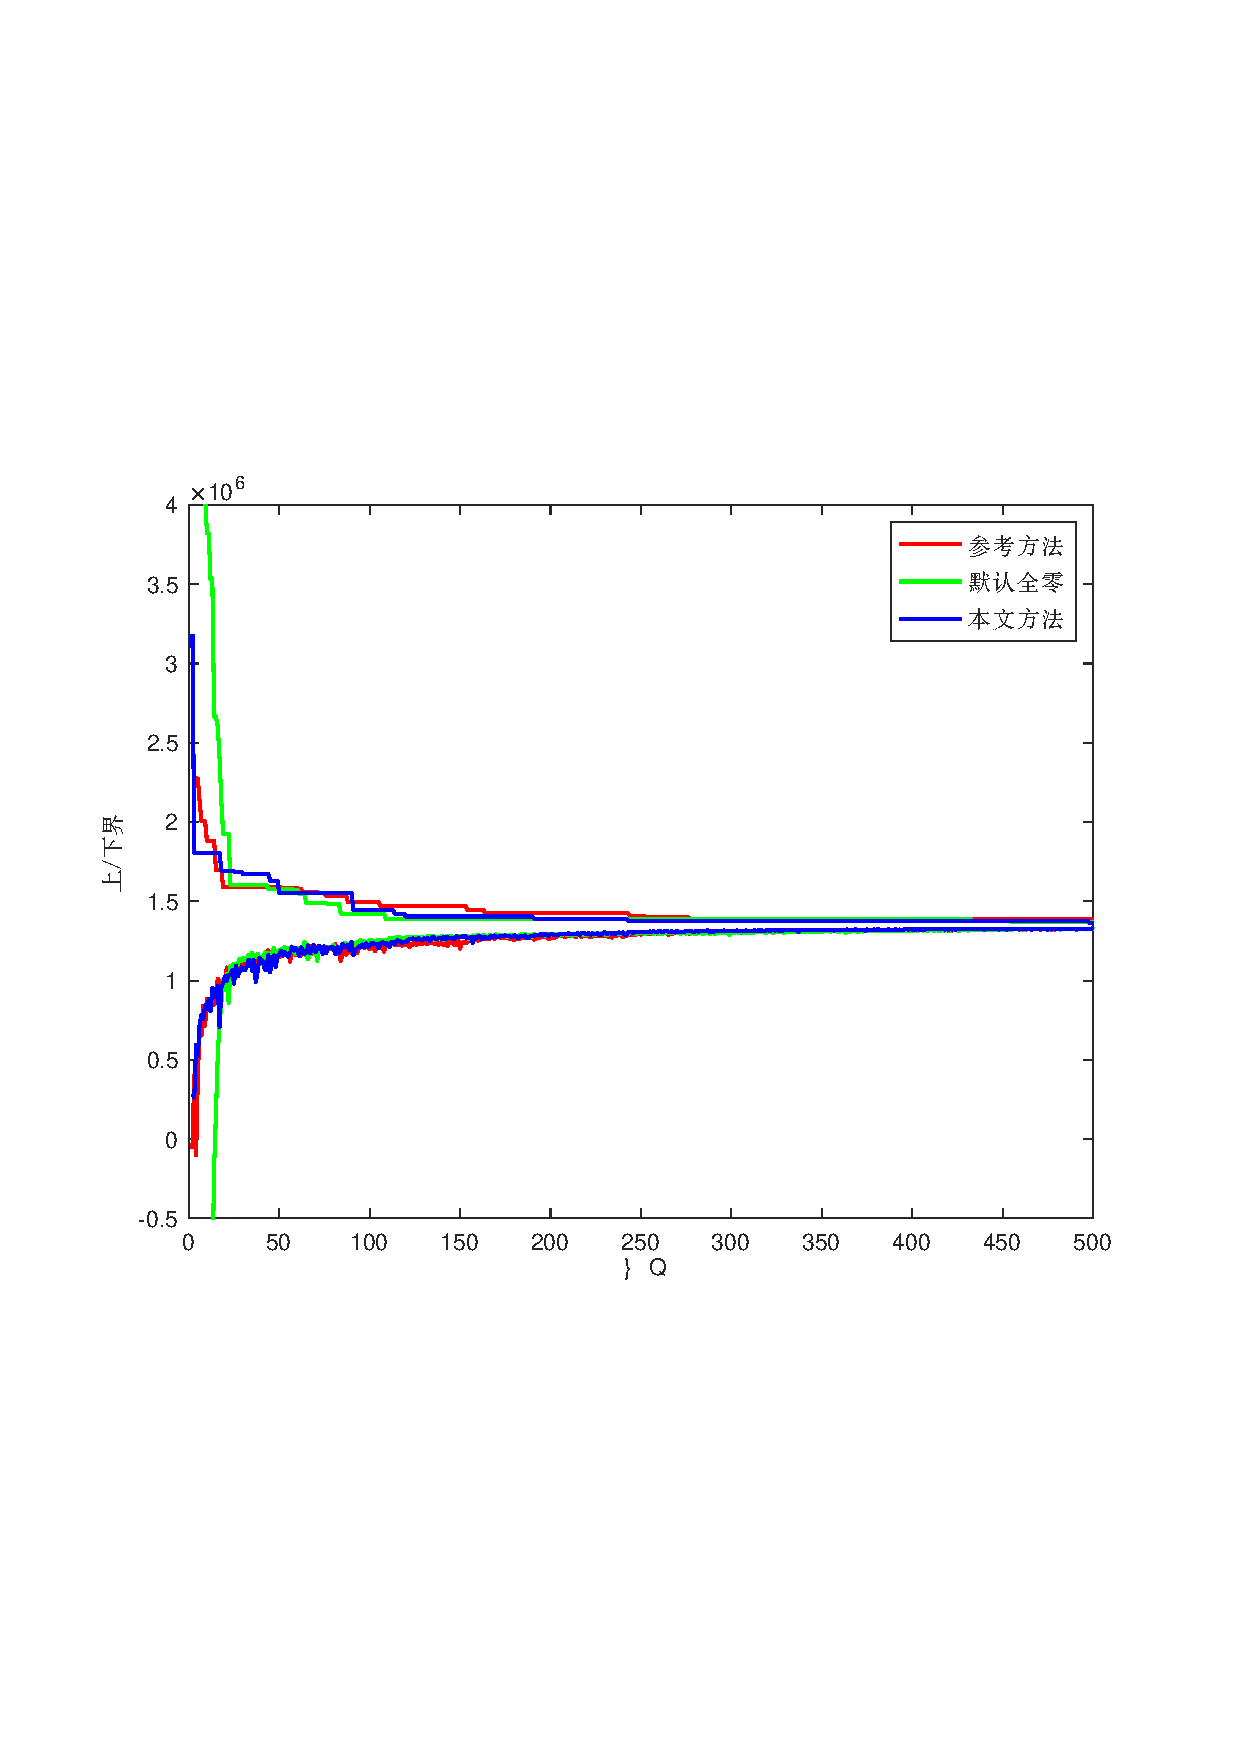
\includegraphics[width=0.47\linewidth]{figures/result_mp_rho0.3.pdf}}
	\caption{乘子初始值的不同策略对优化过程的影响\\Fig~\ref{fig:mp_curves}~ Effect of initialization strategies of the multiplier on the optimization process}
	\label{fig:mp_curves}
	\vspace{-0.35cm} %设置与上面正文的距离
\end{figure}

图\ref{fig:mp_curves}中展示了在不同$\rho$取值的情况下,
算法前500次迭代的结果。
图中绿色曲线表示将全部乘子初始值设置成0的结果,
红色表示文献\cite{yun2015}使用的乘子初始化方法,
蓝色曲线表示本文使用的乘子初始化方法。
从整体优化的趋势来看,
三种方法的优化曲线都呈现良好的收敛趋势,
最终上下界都收敛只最优解附近。
然而,效果最差的初始乘子方法是默认全零方法,
该方法的初始gap值非常大,
并且在$\rho=0.05$的情况下迭代次数最多。
虽然该方法的前期gap值非常差,
但可以快速收敛,
并且在所有测试中下界收敛效果最好。
对比文献\cite{yun2015}的方法,
本文的方法在LR迭代的第一次迭代时得到的上界更大,
但可以快速下降。
本文方法获得的上界结果不如文献\cite{yun2015}的方法,
但获取下界的效果更好,
体现在下界初始波动更小,
获得的下界值更高。
为了方便展示优化曲线的主体部分,
图\ref{fig:mp_curves}忽略了默认全零方法前几次迭代的下界结果,
该下界结果的量级在$-10^{7}$左右。
相比之下,其他两种方法的初始下界均在0附近。

得益于良好的迭代策略,
三种方法最后都收敛于最优解附近。
公式(\ref{eq:steplen})展示了拉格朗日乘子步长设置的准则,
对基础乘子更新策略中迭代步长进行了改进,
取消了分母的二次项并设置为一次项。

图\ref{fig:step_curves}展示了算法两种不同乘子更新策略的结果,
同样以49个点的为基准进行测试,
其中默认$R=5$,
参数$\rho$分别取值0.05、0.1、0.2、0.3。
图中红色的曲线表示若公式(\ref{eq:steplen})分母项取二次(即原始步长公式)获得的上下界迭代效果,
蓝色曲线表示公式(\ref{eq:steplen})(即本文使用的改进公式)的效果。
显然,无论是收敛性还是上下界质量,
使用改进公式的效果都十分明显。
产生这样的差异的原因是,
当公式(\ref{eq:steplen})的分母取平方项时,
生成的迭代步长过小,
每次迭代对拉格朗日乘子的修正较小,
因此获取上下界的效果较差。
改进的公式取消了平方操作,
每次迭代的步长较大,乘子更新更为激进,
进而得到了良好的效果。


\begin{figure}[htb] %这里使用的是强制位置,除非真的放不下,不然就是写在哪里图就放在哪里,不会乱动
	\centering  %图片全局居中
	\vspace{-0.35cm} %设置与上面正文的距离
	\subfigtopskip=2pt %设置子图与上面正文或别的内容的距离
	\subfigbottomskip=2pt %设置第二行子图与第一行子图的距离,即下面的头与上面的脚的距离
	\subfigcapskip=-5pt %设置子图与子标题之间的距离
	\subfigure[$\rho=0.05$]{
		\label{fig:step_sub1}
		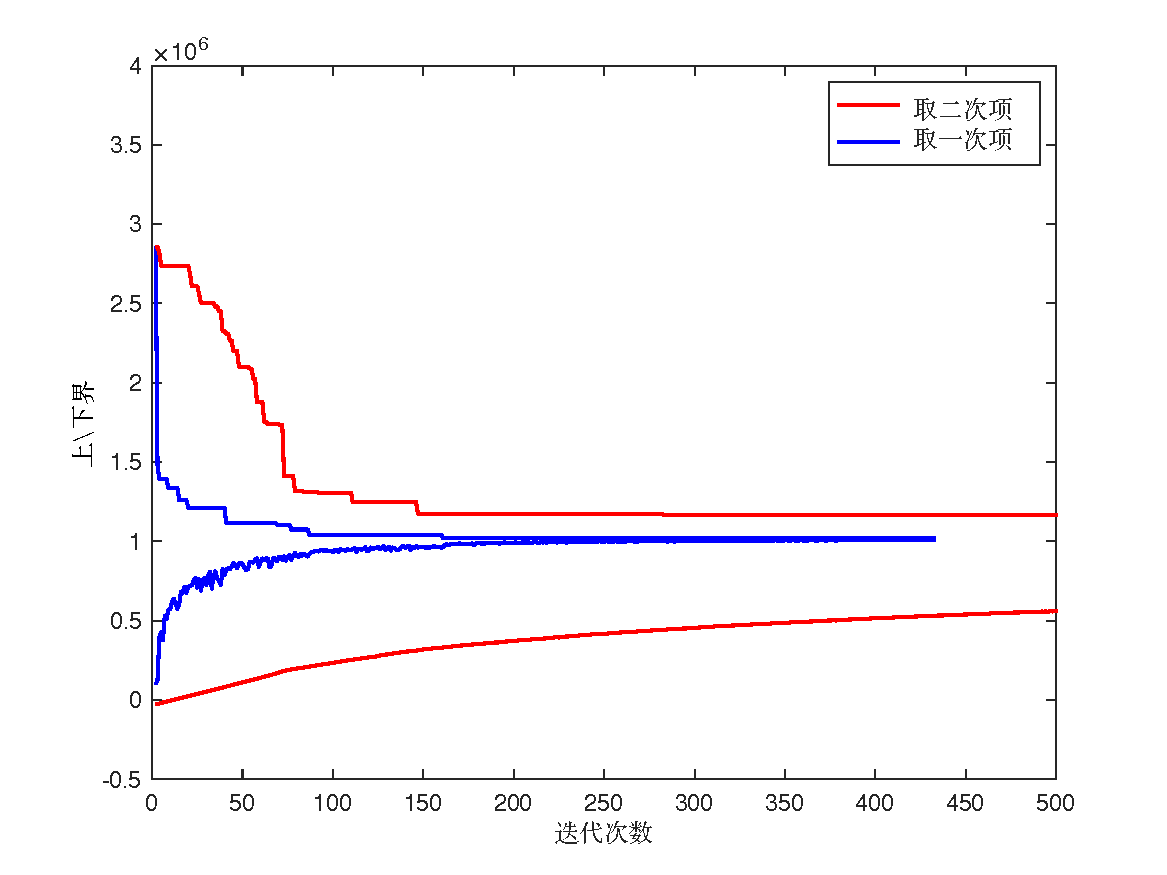
\includegraphics[width=0.47\linewidth]{figures/result_mu_update0.05.pdf}}
	\quad %默认情况下两个子图之间空的较少,使用这个命令加大宽度
	\subfigure[$\rho=0.1$]{
		\label{fig:step_sub2}
		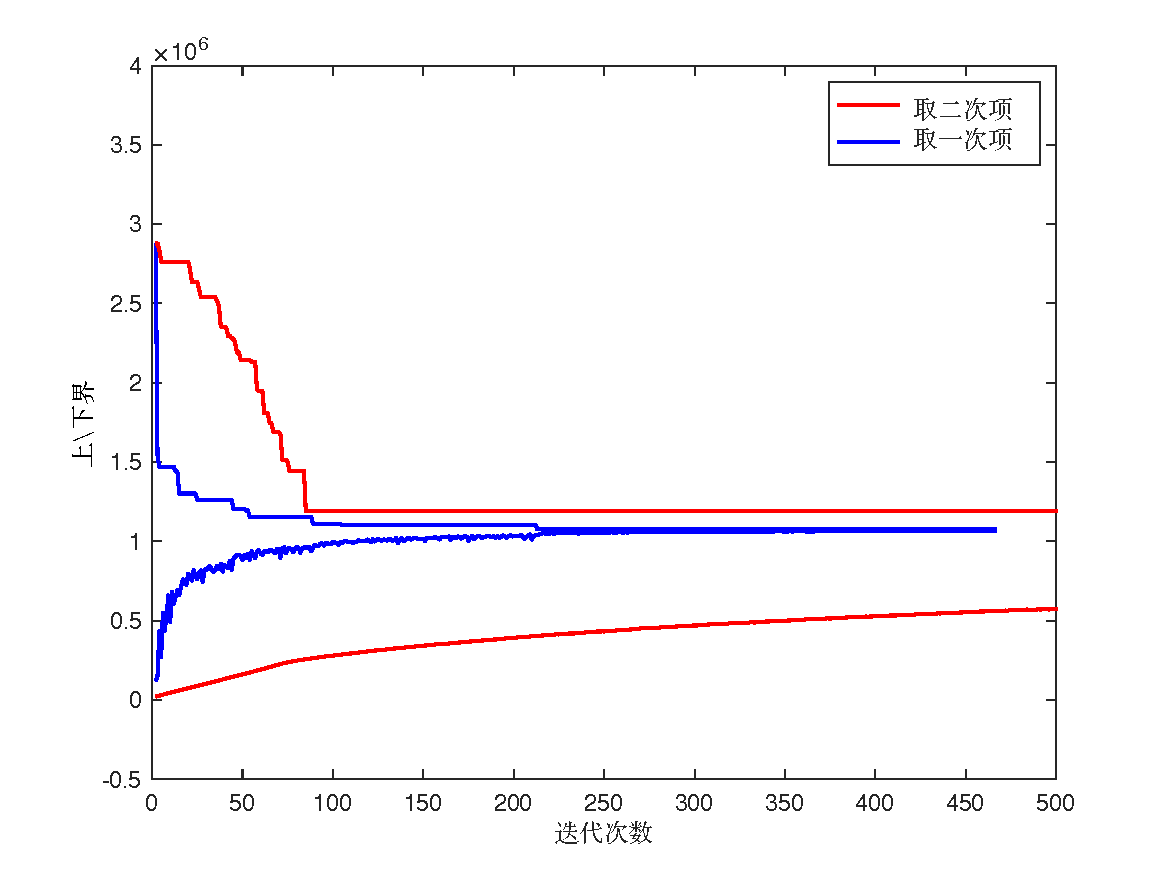
\includegraphics[width=0.47\linewidth]{figures/result_mu_update0.1.pdf}}
	  %这里是空了一行,能够实现强制将四张图分成两行两列显示,而不是放不下图了再换行,使用\\也行。
	\subfigure[$\rho=0.2$]{
		\label{fig:step_sub3}
		% \includegraphics[width=0.47\linewidth]{figures/result_mp_rho0.2.eps}}
		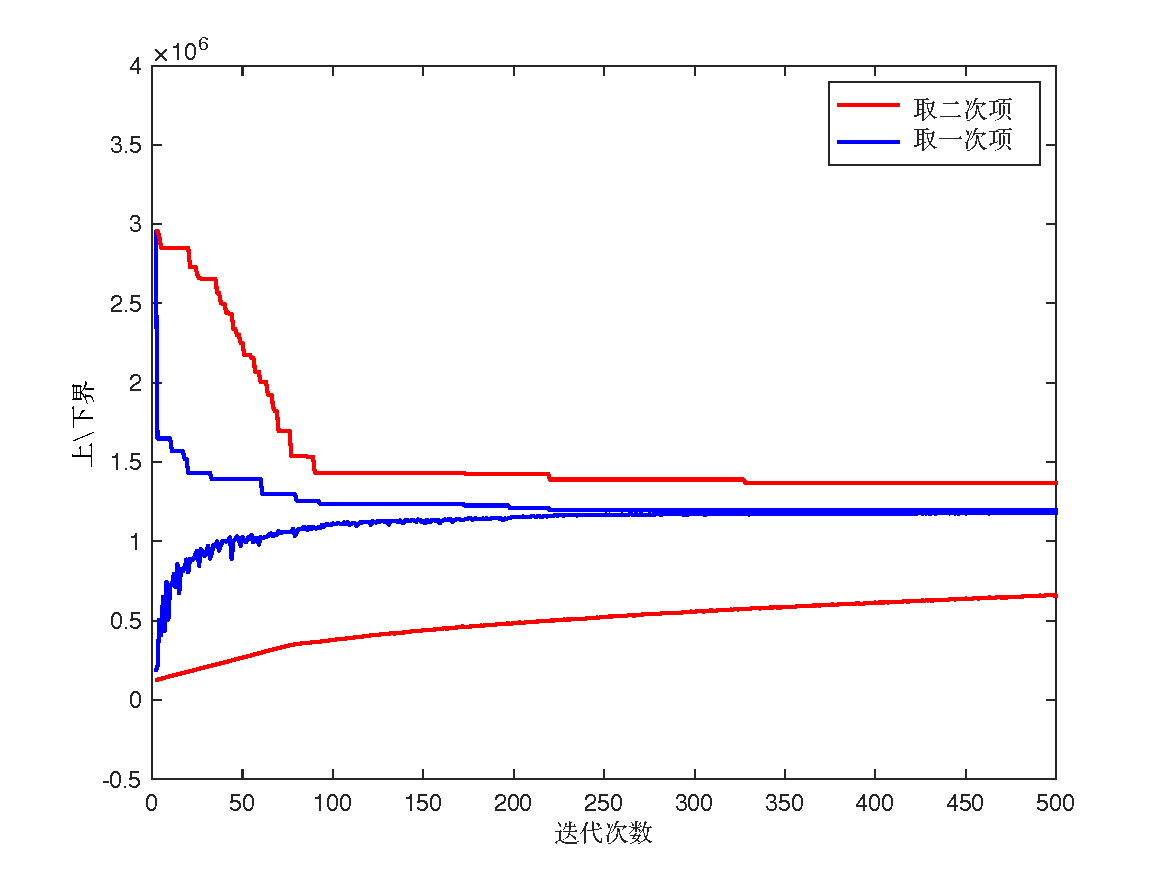
\includegraphics[width=0.47\linewidth]{figures/result_mu_update0.2.pdf}}
	\quad
	\subfigure[$\rho=0.3$]{
		\label{fig:step_sub4}
		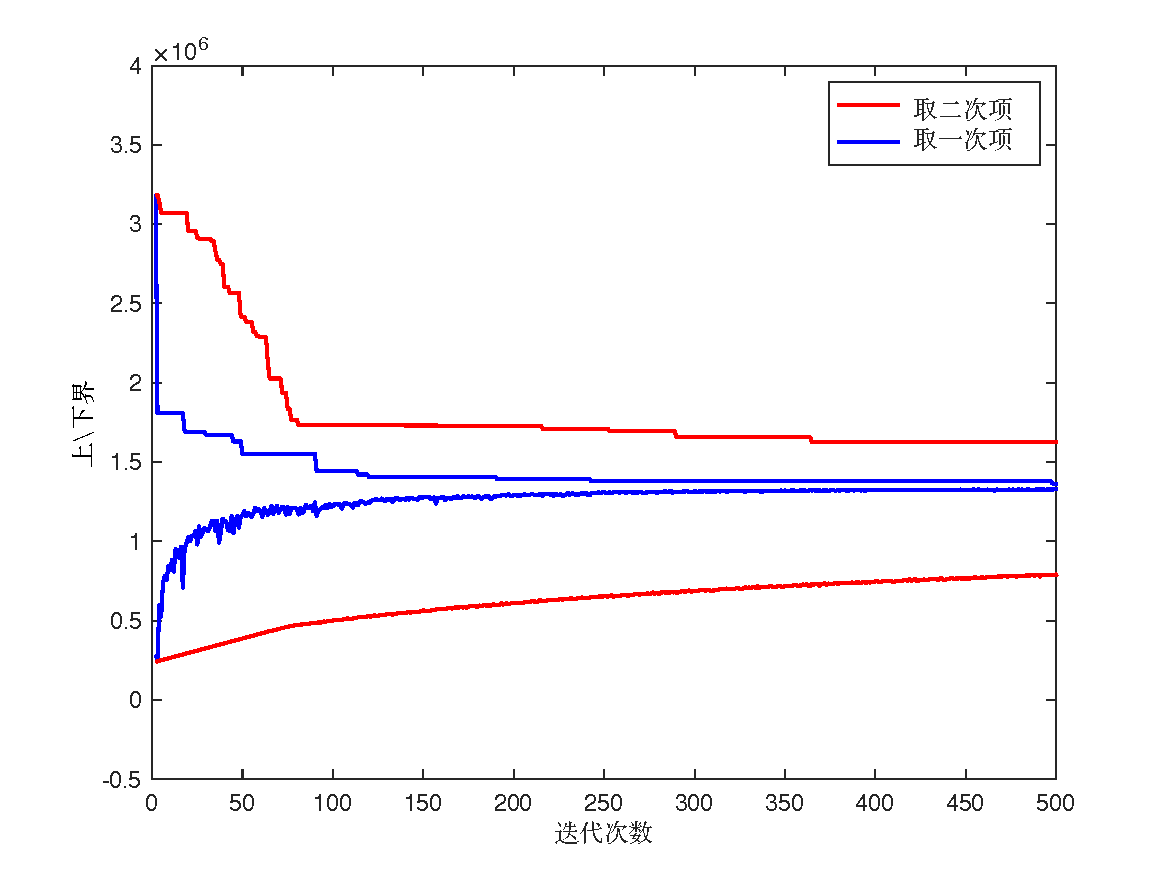
\includegraphics[width=0.47\linewidth]{figures/result_mu_update0.3.pdf}}
	\caption{迭代步长对优化过程的影响\\Fig~\ref{fig:step_curves}~ Effect of step length strategies of the multiplier on the optimization process}
	\label{fig:step_curves}
	\vspace{-0.35cm} %设置与上面正文的距离
\end{figure}


\section{线性化效果讨论}
\label{sec:线性化优势}

本文的第\ref{sec:线性化}节提出了模型的线性化方法,
该方法消除了模型中的二次项,
在理想情况下可降低采用精确方法求解问题的难度。
本节将对比使用Gurobi求解线性模型和非线性模型的性能差距。
求解器参数设置同表\ref{table:参数取值}一致,
测试了15个点的小规模数据集,
其来源于49个点的数据集的前15个点。
设置参数$\rho$分别等于0.05,0.1,0.2,0.3,
参数$R$为大于等于2小于等于10的整数,
求解结果如表\ref{table:线性化结果}所示。
表中上界值为模型的目标函数值,
即目标函数(\ref{eq:obj_model})和目标函数(\ref{eq:l_obj_model}),
gap值为Gurobi返回的gap结果,
求解时间为Gurobi求解时长(秒)。


从表\ref{table:线性化结果}的结果综合来看,
使用Gurobi求解器求解线性模型和非线性模型的困难程度相差不大。
在上述测试中,求解线性模型的平均时间为494.35秒,
求解非线性模型的平均时间为469.79秒;
求解线性模型平均gap值为1.82\%,
非线性模型平均gap值为1.87\%。
对于小规模的15个点的问题,
当参数$\rho$较小时,
求解线性模型相对容易,
当参数$\rho$较大时,
线性化的作用并不明显,
在某些数据测试中,求解线性模型较为简单,
在其他数据测试中,求解非线模型较为简单。

{ \small
\begin{longtable}{ccrrrrrr}
	\caption{非线性模型和线性模型求解结果对比\\Table~\ref{table:线性化结果}~Comparing the results of solving the linear and non-linear models}
    \label{table:线性化结果} \\ % add \\ command to tell LaTeX to start a new line
 
    % Appear table header at the first page as well
    \toprule
	\multirow{2}[0]{*}{$\rho$} & \multirow{2}[0]{*}{$R$} & \multicolumn{3}{c}{非线性模型} & \multicolumn{3}{c}{线性模型} \\
	\cmidrule(r){3-5} \cmidrule(r){6-8}
	&       & \multicolumn{1}{c}{上界值} & \multicolumn{1}{c}{gap} & \multicolumn{1}{c}{时长(s)} & \multicolumn{1}{c}{上界值} & \multicolumn{1}{c}{gap} & \multicolumn{1}{c}{时长(s)} \\
    
	\hline
    \endfirsthead
 
    % Appear the table header at the top of every page
	\multicolumn{8}{r}%
	{{(续\tablename\thetable{})}} \\
    \toprule
	\multirow{2}[0]{*}{$\rho$} & \multirow{2}[0]{*}{$R$} & \multicolumn{3}{c}{非线性模型} & \multicolumn{3}{c}{线性模型} \\
	\cmidrule(r){3-5} \cmidrule(r){6-8}
	&       & \multicolumn{1}{c}{上界值} & \multicolumn{1}{c}{gap} & \multicolumn{1}{c}{时长(s)} & \multicolumn{1}{c}{上界值} & \multicolumn{1}{c}{gap} & \multicolumn{1}{c}{时长(s)} \\
	\hline
	\endhead 
 
    % Appear \hline at the bottom of every page
    \hline
	\multicolumn{3}{l}{{(接续\tablename\ \thetable{})}} \\ 
    \endfoot 
	
	\hline
	\endlastfoot
    % data begins here]
	% Table generated by Excel2LaTeX from sheet '线性化'

			& 2     & 1184928.86 & 0.00\% & 0.07  & 1184928.86 & 0.00\% & 0.08 \\
			& 3     & 664900.02 & 0.00\% & 3.48  & 664900.02 & 0.00\% & 2.83 \\
			& 4     & 644206.22 & 0.00\% & 6.02  & 644206.22 & 0.00\% & 5.47 \\
			& 5     & 643430.51 & 0.00\% & 5.55  & 643430.51 & 0.00\% & 4.52 \\
	  0.05  & 6     & 643401.30 & 0.00\% & 6.55  & 643401.87 & 0.00\% & 4.22 \\
			& 7     & 643401.56 & 0.00\% & 6.03  & 643401.17 & 0.00\% & 3.70 \\
			& 8     & 643401.34 & 0.00\% & 4.57  & 643402.93 & 0.00\% & 3.57 \\
			& 9     & 643409.86 & 0.00\% & 6.67  & 643401.18 & 0.00\% & 3.97 \\
			& 10    & 643401.32 & 0.00\% & 5.30  & 643401.11 & 0.00\% & 5.13 \\
			& 2     & 1736825.35 & 0.00\% & 0.04  & 1736825.35 & 0.00\% & 0.05 \\
			& 3     & 777800.34 & 0.00\% & 11.69 & 777800.34 & 0.00\% & 13.23 \\
			& 4     & 698526.23 & 0.00\% & 509.63 & 698526.23 & 0.10\% & 1000.08 \\
			& 5     & 692637.63 & 0.06\% & 1000.07 & 692637.63 & 0.00\% & 164.69 \\
	  0.1   & 6     & 692205.27 & 0.00\% & 117.82 & 692205.25 & 0.01\% & 138.43 \\
			& 7     & 692175.16 & 0.05\% & 1000.07 & 692174.56 & 0.00\% & 210.79 \\
			& 8     & 692176.10 & 0.00\% & 45.59 & 692174.51 & 0.04\% & 1000.05 \\
			& 9     & 692176.11 & 0.00\% & 44.68 & 692174.55 & 0.00\% & 187.83 \\
			& 10    & 692175.82 & 0.00\% & 50.29 & 692174.53 & 0.04\% & 1000.09 \\
			& 2     & 2719339.96 & 0.00\% & 0.05  & 2719339.96 & 0.00\% & 0.06 \\
			& 3     & 1114008.80 & 0.00\% & 14.36 & 1114008.80 & 0.00\% & 9.11 \\
			& 4     & 845062.91 & 5.40\% & 1000.24 & 845062.91 & 5.92\% & 1000.04 \\
			& 5     & 804766.33 & 2.55\% & 1000.25 & 804766.33 & 2.01\% & 1000.15 \\
	  0.2   & 6     & 798898.18 & 2.19\% & 1000.20 & 798898.18 & 2.03\% & 1000.31 \\
			& 7     & 798124.48 & 1.96\% & 1000.16 & 798124.48 & 1.63\% & 1000.06 \\
			& 8     & 798124.42 & 1.88\% & 1000.07 & 798124.48 & 2.22\% & 1000.13 \\
			& 9     & 798124.48 & 1.66\% & 1000.09 & 798124.48 & 1.64\% & 1000.07 \\
			& 10    & 798124.48 & 1.27\% & 1000.49 & 798124.47 & 1.79\% & 1000.13 \\
			& 2     & 3625538.91 & 0.00\% & 0.06  & 3625538.91 & 0.00\% & 0.07 \\
			& 3     & 1568969.60 & 0.00\% & 70.28 & 1568969.60 & 0.00\% & 36.28 \\
			& 4     & 1068970.09 & 18.97\% & 1000.29 & 1068970.07 & 18.19\% & 1000.22 \\
			& 5     & 946883.17 & 8.00\% & 1000.27 & 949174.41 & 8.29\% & 1000.27 \\
	  0.3   & 6     & 921146.27 & 5.79\% & 1000.63 & 920491.77 & 4.79\% & 1000.21 \\
			& 7     & 914794.24 & 4.68\% & 1000.26 & 914460.06 & 4.34\% & 1000.30 \\
			& 8     & 913246.31 & 4.41\% & 1000.12 & 913246.31 & 4.47\% & 1000.27 \\
			& 9     & 913511.86 & 4.43\% & 1000.25 & 913246.31 & 4.20\% & 1000.13 \\
			& 10    & 913246.31 & 4.08\% & 1000.10 & 913246.31 & 3.88\% & 1000.23 \\

  
	\bottomrule %[2pt] 
\end{longtable}
}


线性化提升求解效率的局限性主要体现在三个方面:
首先,线性化将模型中的二次项消除,
但相应增加了决策变量和等价约束的个数,
其中变量增加数为$O(|I||J|^2)$,
约束增加数为$O(|I||J|^2)$。
这些额外增加的约束使得线性模型求解难度并没有降低太多。
此外,线性化没有改变模型是混合整数规划模型的本质,
因此,增加的约束和变量增加了模型的维度,
使分支定界的过程同样变得复杂。
最后,线性化没有改变问题是NP-hard的本质,
采用精确求解的方法并不适用于大规模问题或者小规模但复杂的问题。

但线性化仍有一定意义,
它提供了一种可能的降低模型求解难度的方法,
在表\ref{table:线性化结果}中,
对于某些数据集,线性模型显著优于非线性模型。
并且在所有测试结果中,
两种模型的上界值相对误差几乎为0,
区别在于证明上界的最优性以及求解所需的时长。
这表明对于线性模型Gurobi可能已经得到了一个近似最优或最优的上界,
Gurobi的大部分计算时间在证明其最优性。
注意到在本问题中,
线性化技术解决的问题是客户的试错序列中的概率递推关系。
而该问题本质上是一个基本最短路问题,
有学者\cite{jepsen}开发了Branch and Cut算法求解最短路问题,
向模型中增加有效割平面的Branch and Cut算法可能会更加适用于线性模型。

\section{算例结果及灵敏度分析}
\label{sec:算例结果}
本章的前几个小节验证了算法的有效性,
本节将展示算例的选址结果并对模型中重要参数的灵敏度展开分析。
由于本文可以求解150个客户及150个选址点的大规模算例,
因此围绕150个点的数据集展开结果分析。

\subsection{结果展示}
\begin{figure}[!b] % use float package if you want it here
	%\setlength{\abovecaptionskip}{-0.2cm} %调整图片caption与正文之间的间距,table同理。可自己调整。
	\setlength{\belowcaptionskip}{-0.5cm} 
	  \centering
	  \includegraphics[width=0.9\textwidth]{figures/r0.pdf}
	  \caption{算例结果\\Fig~\ref{fig:result_map}~ Results for numerical study}
	  \label{fig:result_map}
\end{figure}

选取150个点的数据集,
设置参数$R=5$,即每个客户最多拥有1个常用节点、3个备用节点和1个虚拟节点,
设置参数$\rho=0.1$。
得到选址方案及网络拓扑结构如图\ref{fig:result_map}所示,
图中蓝色点表示客户点,红色点表示选址点,
图中节点和客户之间的直线表示分配关系,
节点与节点之间的直线表示客户试错策略中两节点的关联性,
两个若节点同时作为客户的相邻等级的常用节点或备用节点,
则两个节点的直线更粗。

在该网络中,
优化结果共选取了9个点作为建设节点,
为全网络中150个客户提供服务。
图\ref{fig:result_map}中所有点的分布呈现西疏东密的趋势,
但在选址结果上,东西两个部分的选址数量接近。
空间上,节点建设更偏向于沿海地区,
中部地区建设节点数量较少。
这与经典选址理论将节点安排在拓扑结构相对中心的位置的经验结果是相悖的,
产生这样现象的原因是节点的损坏概率和建设费用对选址结果的共同作用。

图\ref{fig:result_backup}展示了每个客户的常用节点以及一级至三级备用节点。
空间上,
该图中每个客户与其常用节点的距离相对较近,
当常用节点失效时,客户会前往其余备用节点。
从网络的拓扑结构可发现,
该网络可分成两个独立的网络,
第一个子网络由经度上从左向右4个节点以及相关客户构成,
第二个子网络由其余5个节点和相关客户构成。
产生这样现象的原因是客户和节点的空间位置分布呈现明显的左右分割特征。
由于客户的试错策略以及节点的失效概率,
即使某些备用节点空间上更加靠近客户,
但其并不能成为低等级的备用节点。

\begin{figure}[hbt] %这里使用的是强制位置,除非真的放不下,不然就是写在哪里图就放在哪里,不会乱动
	\centering  %图片全局居中
	\vspace{-0.35cm} %设置与上面正文的距离
	\subfigtopskip=2pt %设置子图与上面正文或别的内容的距离
	\subfigbottomskip=2pt %设置第二行子图与第一行子图的距离,即下面的头与上面的脚的距离
	\subfigcapskip=-5pt %设置子图与子标题之间的距离
	\subfigure[常用节点]{
		\includegraphics[width=0.47\linewidth]{figures/r1.pdf}}
	\quad %默认情况下两个子图之间空的较少,使用这个命令加大宽度
	\subfigure[一级备用]{
		\includegraphics[width=0.47\linewidth]{figures/r2.pdf}}
	  %这里是空了一行,能够实现强制将四张图分成两行两列显示,而不是放不下图了再换行,使用\\也行。
	\subfigure[二级备用]{
		% \includegraphics[width=0.47\linewidth]{figures/result_mp_rho0.2.eps}}
		\includegraphics[width=0.47\linewidth]{figures/r3.pdf}}
	\quad
	\subfigure[三级备用]{
		\includegraphics[width=0.47\linewidth]{figures/r4.pdf}}
	\caption{客户的常用节点和备用节点\\Fig~\ref{fig:result_backup}~ Primary and backup nodes for customers}
	\label{fig:result_backup}
	\vspace{-0.2cm} %设置与上面正文的距离
\end{figure}

\vspace{1ex}
\subsection{参数\texorpdfstring{$\rho$}{p}灵敏度分析}
参数$\rho$控制节点的失效概率,
本小节分析了在参数$R=5$的情况下,
参数$\rho$的取值对选址结果和成本的影响。
其中,参数$\rho$取0.1只0.9之间,间隔为0.1的值。
相关选址结果及成本如表\ref{table:sens_rho}所示。
在本文中,惩罚成本计算在期望运输成本中(参考第\ref{cha:model}章模型目标函数),
为了分析成本的构成及变化情况,
本小节将期望运输成本拆分成运输成本和惩罚成本。

\begin{table}[htbp]
    \setlength{\abovecaptionskip}{-0.05cm} %调整图片caption与正文之间的间距,table同理。可自己调整。
    \setlength{\belowcaptionskip}{-0.2cm} 
    \centering
    \renewcommand\arraystretch{0.9}
    \caption{不同参数$\rho$取值的选址结果。
    \\Table~\ref{table:sens_rho}~Results for different $\rho$.}
	\resizebox{\linewidth}{!}{
		\small{
			\begin{tabular}{clcccc}
				\toprule %[2pt]设置线宽 
				\multirow{2}[0]{*}{$\rho$} & \makecell[c]{\multirow{2}[0]{*}{选址方案}} & \multirow{2}[0]{*}{总成本} & \multirow{2}[0]{*}{固定成本} & \multicolumn{2}{c}{期望运输成本} \\
				\cmidrule{5-6}
					&       &       &       & 运输成本  & 惩罚成本 \\
				\midrule
				0.1 & 	81,94,120,123,127,131,141,142,150	& 2435470.40	& 870000.00	& 1564493.34	& 977.06 \\
				0.2 & 	81,94,112,120,123,126,127,131,142,150	& 2663160.76	& 1090000.00	& 1562646.61	& 10514.15 \\
				0.3 & 	81,86,94,120,123,127,131,132,138,142,150	& 2898709.21	& 1140000.00	& 1694377.11	& 64332.10 \\
				0.4 & 	81,94,95,120,122,132,142,143,150	& 3306483.46	& 1020000.00	& 2126422.07	& 160061.38 \\
				0.5 & 	86,88,94,112,120,122,126,135,142	& 3804266.94	& 1170000.00	& 2347124.47	& 287142.46 \\
				0.6 & 	18,65,81,120,126,135,137,140,142	& 4075532.71	& 1390000.00	& 2531507.27	& 154025.44 \\
				0.7 & 	8,31,54,57,65,110			& 4464655.64	& 1500000.00	& 2910757.78	& 53897.86 \\
				0.8 & 	27,54,61,65,66,124,126		& 4713189.05	& 1730000.00	& 2889043.65	& 94145.40 \\
				0.9 & 	8,9,43,54,102,122			& 4679935.27	& 1650000.00	& 2960134.85	& 69800.42 \\
				\bottomrule  
			\end{tabular}%
		}
	}
    \label{table:sens_rho}
\end{table}%

随着参数$\rho$增加,
选址节点的数量在不断变化,
且选址方案变化较大。
在相对较小的$\rho$取值下,
结果表明候选点81、94、112、120、122、127、131、142、150更易被选为建设节点,
当$\rho$值较大时,
节点建设方案不固定且变化巨大。
这表明,节点的失效概率影响选址结果,
特别是影响选址建设方案。
在参数$\rho$变化一定程度内,
选址方案变动不大。
当超过一定值时,选址方案随参数的变化发生巨大变动。

综合分析成本,
随着节点的失效概率增加,
系统的总成本呈现增加趋势,
为可视化各项成本的变动,
图\ref{fig:sens_rho}展示了各项成本随参数$\rho$变化的曲线。
首先,总成本曲线表明系统的总成本随$\rho$的增加而增加。
其次,三项成本之间的权衡曲线表明,
随着节点失效概率的增长,
最开始,系统不得不建设更多的设施、产生更多的固定成本以缓和总成本的增加,
接着运输成本大幅上升,系统不得不缩减固定成本以降低总成本增长趋势。
运输成本随节点失效概率的增加而增加,
相应结果下固定成本下降,
产生``效益背反''现象。
最后,系统的惩罚成本随节点的失效概率的增加先上升后下降,
同样为系统的成本权衡结果。
为了降低总成本,系统不得不牺牲一部分的可靠性,
换取相对较低的总成本。

\begin{figure}[hbt] % use float package if you want it here
	%\setlength{\abovecaptionskip}{-0.2cm} %调整图片caption与正文之间的间距,table同理。可自己调整。
	\setlength{\belowcaptionskip}{-0.5cm} 
	  \centering
	  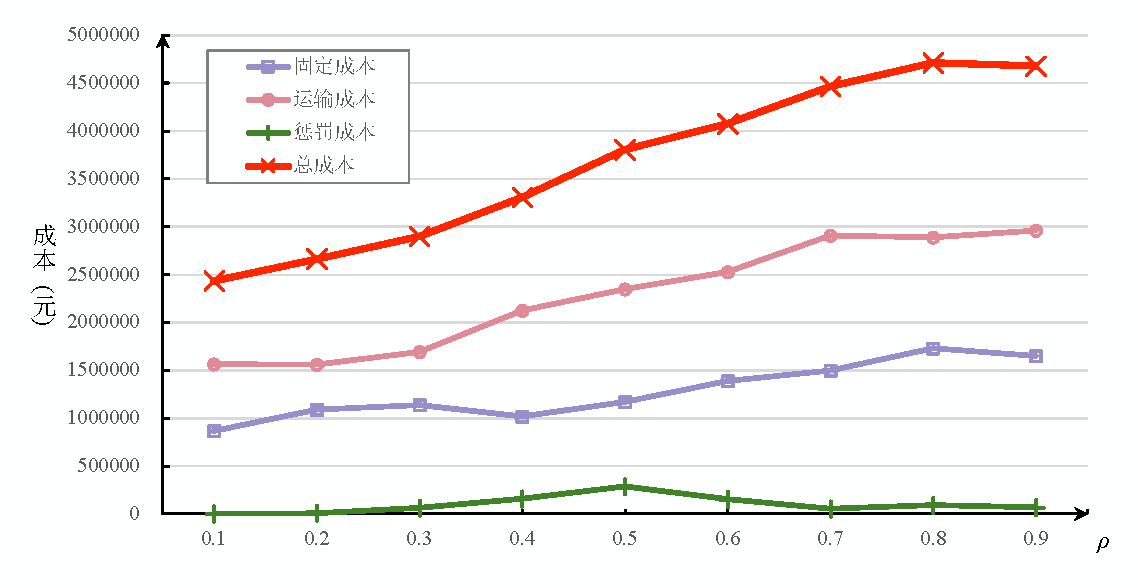
\includegraphics[width = 0.9 \textwidth]{figures/sens_rho.pdf}
	  \caption{成本随$\rho$变动的权衡曲线\\
	  Fig~\ref{fig:sens_rho}~ Trade-off curves for the variation of each cost with $\rho$}
	  \label{fig:sens_rho}
\end{figure}

\subsection{参数\texorpdfstring{$R$}{R}灵敏度分析}
本小节将分析参数$R$对选址结果的影响,
设置参数$\rho=0.1$,
参数$R$等于2至10的不同整数值,
即每个客户拥有0个至8个备用节点。
参数$R$控制每个客户拥有的常用节点、备用节点和虚拟节点的总数量。
已知每个客户必须拥有一个虚拟节点和一个常用节点,
则$R$的最小值为2。
表\ref{table:sens_r}展示了不同$R$取值下的选址方案和成本构成。



\begin{table}[htbp]
    \setlength{\abovecaptionskip}{-0.05cm} %调整图片caption与正文之间的间距,table同理。可自己调整。
    \setlength{\belowcaptionskip}{-0.2cm} 
    \centering
    \renewcommand\arraystretch{0.9}
    \caption{不同参数$R$取值的选址结果。
    \\Table~\ref{table:sens_r}~Results for different $R$.}
	\resizebox{\linewidth}{!}{
		\small{
			\begin{tabular}{clcccc}
				\toprule %[2pt]设置线宽 
				\multirow{2}[0]{*}{$R$} & \makecell[c]{\multirow{2}[0]{*}{选址方案}} & \multirow{2}[0]{*}{总成本} & \multirow{2}[0]{*}{固定成本} & \multicolumn{2}{c}{期望运输成本} \\
				\cmidrule{5-6}
					&       &       &       & 运输成本  & 惩罚成本 \\
				\midrule
				2&	8,13,54,66					&4670884.11	&1620000	&1984693.82	&1066190.29 \\
				3&	81,94,95,120,127,142,149,150			&2591989.01	&890000		&1510101.65	&191887.36\\
				4&	81,94,120,123,127,131,141,142,149,150		&2410503.11	&1000000	&1395715.25	&14787.86\\
				5&	81,94,120,123,127,131,141,142,149,150		&2397743.05	&1000000	&1396787.65	&955.40\\
				6&	79,81,94,120,123,127,131,138,141,142,150	&2398531.47	&1130000	&1268481.33	&50.14\\
				7&	81,94,120,123,127,131,138,141,142,150		&2402250.12	&1000000	&1402247.14	&2.98\\
				8&	81,94,120,123,127,131,141,142,149,150		&2396859.14	&1000000	&1396858.93	&0.21\\
				9&	81,94,120,123,127,131,141,142,149,150		&2396858.96	&1000000	&1396858.95	&0.01\\
				10&	81,94,120,123,127,131,141,142,149,150		&2396858.95	&1000000	&1396858.95	&0.00\\
				\bottomrule  
			\end{tabular}%
		}
	}
    \label{table:sens_r}
\end{table}%

首先分析选址方案的变化,
当$R=2$时,此时问题的退化成UFL问题,
此时选址的数量较少,但固定成本较高。
由于未向任何客户指派备用节点,因此$R=2$时方案的惩罚成本非常高。
当$R=3$时,即向每个客户指派1个备用节点,
惩罚成本大幅度下降。
这说明向客户即便向每个客户仅指派1个备用节点,
也能显著提高网络的可靠性。
随着每个客户备用节点数量的增加,
惩罚成本下降。
最终选址方案趋于稳定,总成本不再明显变化。
选址方案受参数$R$的影响较小,
结果鲁棒性较强,
表明在81、94、120、123、127、131、142、149、150等选址点处建设设施具有可靠性。

其次,相关成本随$R$的变化如图\ref{fig:sens_r}所示,
随着参数$R$的增加,
网络的总成本逐渐下降并趋于稳定。
产生该现象的原因是为每个客户安排常用节点,
降低了惩罚成本,
当惩罚成本几乎不变时,
选址结果同样不会变动。
图\ref{fig:sens_r}中展示的优化曲线表明为每个客户安排一个常用节点和三个备用节点时,
该网络已经变得足够可靠,
再向其添加备用节点对选址总成本不会产生较大的影响。

\begin{figure}[hbt] % use float package if you want it here
	%\setlength{\abovecaptionskip}{-0.2cm} %调整图片caption与正文之间的间距,table同理。可自己调整。
	\setlength{\belowcaptionskip}{-0.5cm} 
	  \centering
	  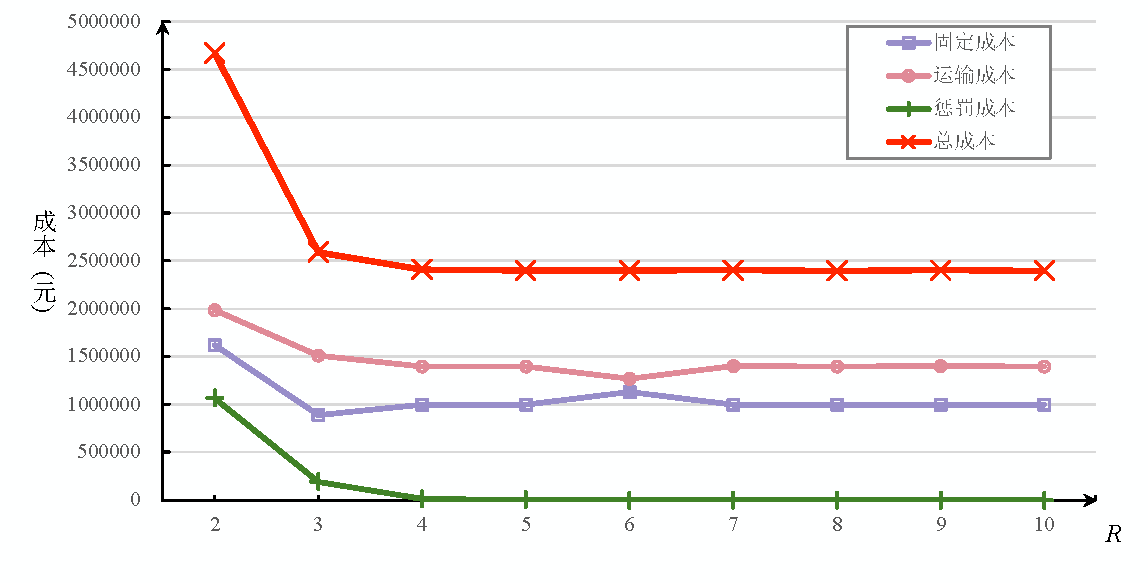
\includegraphics[width = 0.9 \textwidth]{figures/sens_r.pdf}
	  \caption{成本随$R$变动的权衡曲线\\
	  Fig~\ref{fig:sens_r}~ Trade-off curves for the variation of each cost with $R$}
	  \label{fig:sens_r}
\end{figure}

在本算例的灵敏度分析中,
系统的可靠性随备用节点个数的增加而增加。
然而,仅依靠增加备用节点个数以提高网络可靠性是有边界的。
超过此边界后,
再增加节点也很难影响选址方案和总成本。
在本算例中,$R=5$是每个客户拥有的最佳节点数量。
若$R$低于此值,网络变得不可靠,
若$R$高于此值,增加了运算量的同时对网络选址结果不产生较大影响。

\section{本章小结}
\label{sec:本章小结5}
本章的主要内容为数值实验和算例分析。
首先采用经典选址数据集构造了数值实验的算例,
对比分析了LR-ILS算法与商业求解器的求解结果。
结果表明,
根据问题定制的LR-ILS算法可以在短时间内获得近似最优解,
并且可以求解150个客户与150个候选位置的大规模数据。
在绝大多数算例中,
LR-ILS求解结果和求解时间显著优于求解器。
此外,数值实验还针对LR-ILS算法的各种算子性能和算法设计展开了分析,
特别是求解模型上界、下界的性能,
以及多种乘子初始化和更新方法的效果。
数值实验还讨论了模型线性化的效果,
对比分析使用求解器求解非线性模型和线性模型的差异。
最后,给出了算例选址结果,以及重要参数的灵敏度分析结果。
值得注意的是,
由于该算法使用了元启发式算子,
算法本质上带有随机性,
因此会造成运行最终结果中上界不稳定的情况。
但是,算法的下界提供了上界质量的证明。

